\documentclass[11pt,a4paper]{article}
\usepackage[margin=2.2cm]{geometry}
\usepackage{amsmath,amssymb}
\usepackage{graphicx}
\usepackage{booktabs}
\usepackage{tabularx}
\usepackage{caption}
\usepackage{xcolor}
\usepackage{hyperref}
\usepackage{fancyhdr}
\usepackage{microtype}
\usepackage{titlesec}
\usepackage{enumitem}
\usepackage{float}

\definecolor{primary}{RGB}{27,68,120}
\definecolor{darkgray}{RGB}{60,60,60}
\hypersetup{colorlinks=true,linkcolor=primary,citecolor=primary,urlcolor=primary,
  pdftitle={Simulation and Validation of a Fixed-Bed Downdraft Wood Gasifier - Batch 09}}
\pagestyle{fancy}\fancyhf{}
\fancyhead[L]{\small\textcolor{darkgray}{Fixed-bed downdraft gasifier simulation}}
\fancyhead[R]{\small\textcolor{darkgray}{Batch 09}}
\fancyfoot[C]{\thepage}
\titleformat{\section}{\Large\bfseries\color{primary}}{\thesection}{1em}{}
\titleformat{\subsection}{\large\bfseries\color{primary}}{\thesubsection}{1em}{}
\graphicspath{{figures/}}
\setlist{itemsep=2pt,topsep=4pt}
% AUTO-GENERATED by scripts/make_report_tables.py - do not edit
\newcommand{\RUwall}{114.4}
\newcommand{\RetaB}{0.474}
\newcommand{\RetaWG}{0.142}
\newcommand{\RAFRstoich}{6.22}
\newcommand{\RLHVwood}{18.17}
\newcommand{\RERref}{0.35}
\newcommand{\RERcal}{0.30}
\newcommand{\RFormula}{CH$_{1.53}$O$_{0.62}$N$_{0.0034}$}
\newcommand{\RTthroatRef}{1604}
\newcommand{\RTadRef}{1345}
\newcommand{\RTsZeroRef}{1554}
\newcommand{\RTexitRef}{838}
\newcommand{\RTtenRef}{1172}
\newcommand{\RTfiveRef}{1332}
\newcommand{\RdTgsMax}{155}
\newcommand{\RzEquil}{7.6}
\newcommand{\RCOexitRef}{21.30}
\newcommand{\RHtwoExitRef}{13.49}
\newcommand{\RCOtwoExitRef}{9.03}
\newcommand{\RCHfourExitRef}{1.05}
\newcommand{\RNtwoExitRef}{55.13}
\newcommand{\RCOthroatRef}{13.74}
\newcommand{\RHtwoThroatRef}{9.24}
\newcommand{\RCOtwoThroatRef}{12.59}
\newcommand{\RHtwoOinRef}{23.6}
\newcommand{\RHtwoOoutRef}{17.7}
\newcommand{\RXcRef}{50.3}
\newcommand{\RzHalfRef}{2.4}
\newcommand{\RdpExitRef}{1.98}
\newcommand{\RFlowRef}{45.4}
\newcommand{\RLHVRef}{4.52}
\newcommand{\RCGERef}{56.3}
\newcommand{\RWallkWRef}{14.0}
\newcommand{\RWallPctRef}{13.8}
\newcommand{\RQinRef}{101.3}
\newcommand{\RCalMAE}{0.43}
\newcommand{\RCalRMSE}{0.53}
\newcommand{\RCalMAEJ}{0.46}
\newcommand{\RCalRMSEJ}{0.57}
\newcommand{\RCalTthroat}{1422}
\newcommand{\RCalTad}{1164}
\newcommand{\RCalXc}{17.0}
\newcommand{\RCalCGE}{48.1}
\newcommand{\RCalTexit}{787}
\newcommand{\RCalFlow}{39.4}
\newcommand{\RTempMAE}{93}
\newcommand{\RTempRMSE}{103}
\newcommand{\RTempBias}{-52}
\newcommand{\RTempMAEJ}{121}
\newcommand{\RTempRMSEJ}{132}
\newcommand{\RTwoDaxisTexit}{1292}
\newcommand{\RTwoDwallTexit}{558}
\newcommand{\RTwoDaxisTfive}{1448}
\newcommand{\RTwoDwallTfive}{1250}
\newcommand{\RTwoDmixT}{966}
\newcommand{\RTwoDwallkW}{10.5}
\newcommand{\RTwoDCOaxis}{25.4}
\newcommand{\RTwoDCOwall}{20.4}
\newcommand{\RTwoDHtwoaxis}{15.7}
\newcommand{\RTwoDHtwowall}{13.0}
\newcommand{\RTwoDXcAxisEleven}{99.8}
\newcommand{\RTwoDXcWallExit}{29.9}
\newcommand{\RTwoDXcAxisFive}{89.5}
\newcommand{\RTwoDmixCO}{22.76}
\newcommand{\RTwoDmixHtwo}{14.29}
\newcommand{\RTwoDmixCOtwo}{8.34}
\newcommand{\RTwoDmixNtwo}{53.59}
\newcommand{\RTwoDcells}{12}
\newcommand{\RTwoDnz}{111}
\newcommand{\REnergyResidual}{-0.07}
\newcommand{\RWGSfastCO}{9.0}
\newcommand{\RWGSfastHtwo}{22.8}
\newcommand{\RWGSfastCOtwo}{18.0}
\newcommand{\RRuntime}{29}
\newcommand{\RWallShare}{71}
\newcommand{\RRxnShare}{29}
\newcommand{\RSensDrop}{19.9}
\newcommand{\RBaseTtwelve}{1129}
\newcommand{\RMAECO}{1.42}
\newcommand{\RRMSECO}{1.74}
\newcommand{\RBiasCO}{-0.15}
\newcommand{\RRsqCO}{-1.99}
\newcommand{\RWithinCO}{7}
\newcommand{\RStdCO}{1.00}
\newcommand{\RMAExCO}{1.41}
\newcommand{\RBiasxCO}{+0.02}
\newcommand{\RMAEHtwo}{2.01}
\newcommand{\RRMSEHtwo}{2.73}
\newcommand{\RBiasHtwo}{-1.87}
\newcommand{\RRsqHtwo}{-0.55}
\newcommand{\RWithinHtwo}{5}
\newcommand{\RStdHtwo}{2.19}
\newcommand{\RMAExHtwo}{2.21}
\newcommand{\RBiasxHtwo}{-2.06}
\newcommand{\RMAECOtwo}{0.62}
\newcommand{\RRMSECOtwo}{0.78}
\newcommand{\RBiasCOtwo}{-0.19}
\newcommand{\RRsqCOtwo}{0.04}
\newcommand{\RWithinCOtwo}{7}
\newcommand{\RStdCOtwo}{0.80}
\newcommand{\RMAExCOtwo}{0.68}
\newcommand{\RBiasxCOtwo}{-0.19}
\newcommand{\RMAECHfour}{0.15}
\newcommand{\RRMSECHfour}{0.16}
\newcommand{\RBiasCHfour}{-0.13}
\newcommand{\RRsqCHfour}{-1.47}
\newcommand{\RWithinCHfour}{3}
\newcommand{\RStdCHfour}{0.10}
\newcommand{\RMAExCHfour}{0.16}
\newcommand{\RBiasxCHfour}{-0.16}
\newcommand{\RMAENtwo}{2.84}
\newcommand{\RRMSENtwo}{3.07}
\newcommand{\RBiasNtwo}{+2.31}
\newcommand{\RRsqNtwo}{-0.66}
\newcommand{\RWithinNtwo}{8}
\newcommand{\RStdNtwo}{2.39}
\newcommand{\RMAExNtwo}{2.95}
\newcommand{\RBiasxNtwo}{+2.36}
\newcommand{\RMAELHV}{0.30}
\newcommand{\RRMSELHV}{0.36}
\newcommand{\RBiasLHV}{-0.27}
\newcommand{\RRsqLHV}{-1.21}
\newcommand{\RWithinLHV}{7}
\newcommand{\RStdLHV}{0.24}
\newcommand{\RMAExLHV}{0.32}
\newcommand{\RBiasxLHV}{-0.27}
\newcommand{\RImpliedFeedMin}{23.0}
\newcommand{\RImpliedFeedMax}{28.3}
\newcommand{\RFlowRatioMin}{66}
\newcommand{\RFlowRatioMax}{81}
\newcommand{\RRunTthroatMin}{1422}
\newcommand{\RRunTthroatMax}{1700}
\newcommand{\REffChipA}{63.6}
\newcommand{\ROptChipA}{10}
\newcommand{\REffOptChipA}{63.3}
\newcommand{\RUChipA}{114}
\newcommand{\REffChipB}{54.6}
\newcommand{\ROptChipB}{11}
\newcommand{\REffOptChipB}{54.4}
\newcommand{\RUChipB}{114}
\newcommand{\REffChipC}{50.5}
\newcommand{\ROptChipC}{12}
\newcommand{\REffOptChipC}{50.2}
\newcommand{\RUChipC}{114}
\newcommand{\REffMCA}{62.8}
\newcommand{\ROptMCA}{11}
\newcommand{\REffOptMCA}{62.5}
\newcommand{\RUMCA}{114}
\newcommand{\REffMCB}{54.6}
\newcommand{\ROptMCB}{11}
\newcommand{\REffOptMCB}{54.4}
\newcommand{\RUMCB}{114}
\newcommand{\REffMCC}{47.1}
\newcommand{\ROptMCC}{12}
\newcommand{\REffOptMCC}{46.9}
\newcommand{\RUMCC}{114}
\newcommand{\REffLossA}{66.1}
\newcommand{\ROptLossA}{22}
\newcommand{\REffOptLossA}{66.1}
\newcommand{\RULossA}{35}
\newcommand{\REffLossB}{58.8}
\newcommand{\ROptLossB}{14}
\newcommand{\REffOptLossB}{58.5}
\newcommand{\RULossB}{76}
\newcommand{\REffLossC}{53.7}
\newcommand{\ROptLossC}{11}
\newcommand{\REffOptLossC}{53.5}
\newcommand{\RULossC}{125}
\newcommand{\REffAngleA}{57.3}
\newcommand{\ROptAngleA}{8}
\newcommand{\REffOptAngleA}{57.0}
\newcommand{\RUAngleA}{114}
\newcommand{\REffAngleB}{54.6}
\newcommand{\ROptAngleB}{11}
\newcommand{\REffOptAngleB}{54.4}
\newcommand{\RUAngleB}{114}
\newcommand{\REffAngleC}{51.6}
\newcommand{\ROptAngleC}{18}
\newcommand{\REffOptAngleC}{51.5}
\newcommand{\RUAngleC}{114}
\newcommand{\REffAirA}{54.6}
\newcommand{\ROptAirA}{11}
\newcommand{\REffOptAirA}{54.4}
\newcommand{\RUAirA}{114}
\newcommand{\REffAirB}{60.0}
\newcommand{\ROptAirB}{12}
\newcommand{\REffOptAirB}{59.7}
\newcommand{\RUAirB}{114}
\newcommand{\REffAirC}{65.9}
\newcommand{\ROptAirC}{12}
\newcommand{\REffOptAirC}{65.6}
\newcommand{\RUAirC}{114}
\newcommand{\RAFRCGElo}{46.6}
\newcommand{\RAFRCGEhi}{69.8}
\newcommand{\RAFRTlo}{1385}
\newcommand{\RAFRThi}{1786}
\newcommand{\RAFRXclo}{11}
\newcommand{\RAFRXchi}{99}
\newcommand{\RAFRLHVmin}{4.38}
\newcommand{\RAFRLHVmax}{4.72}
\newcommand{\RFeedFlowLo}{28.9}
\newcommand{\RFeedFlowHi}{58.2}
\newcommand{\RFeedCGElo}{53.8}
\newcommand{\RFeedCGEhi}{55.2}
\newcommand{\RFeedTlo}{669}
\newcommand{\RFeedThi}{938}

\newcommand{\dd}{\mathrm{d}}
\makeatletter\newcommand{\tabinput}[1]{\@@input #1 }\makeatother

\begin{document}

\begin{titlepage}
\centering
\vspace*{2cm}
{\LARGE\bfseries\color{primary} Simulation and Validation of a Fixed-Bed Downdraft Wood Gasifier\par}
\vspace{0.6cm}
{\large One-dimensional kinetic model, two-dimensional axisymmetric extension and parametric study,\\ benchmarked against Jayah et al.\ (2003)\par}
\vspace{2cm}
\small\begin{tabular}{rl}
\textbf{Course:} & Gasification \& Reforming Processes --- Fixed-Bed Gasifier assignment\\[2pt]
\textbf{Batch:} & Batch 09\\[2pt]
\textbf{Reference paper:} & T.H.\ Jayah, L.\ Aye, R.J.\ Fuller, D.F.\ Stewart (2003),\\
 & \emph{Computer simulation of a downdraft wood gasifier for tea drying},\\
 & Biomass and Bioenergy 25(5), 459--469. doi:10.1016/S0961-9534(03)00037-0\\[2pt]
\textbf{Code:} & Python (NumPy, SciPy, Matplotlib); repository and \texttt{run\_simulation.py}\\[2pt]
\textbf{Date:} & October 2026\\
\end{tabular}
\vfill
\end{titlepage}

\tableofcontents
\newpage

%=====================================================================
\section{Abstract}
The 80\,kW$_\text{th}$ throat-type downdraft gasifier built by the NERD Centre (Sri Lanka) for tea drying and studied by Jayah et al.\ (2003) was simulated in Python. A throat sub-model (all oxygen consumed by the volatiles, water-gas-shift equilibrium, temperature from an enthalpy balance anchored to the paper's own throat value) feeds a steady one-dimensional kinetic model of the 22\,cm conical reduction zone with four reactions (Boudouard, water-gas, methanation, water-gas shift), separate gas and char temperatures, shrinking particles and wall heat loss. A two-dimensional axisymmetric extension resolves radial dispersion of heat and species to give the required contour plots.

Three parameters were calibrated: the wall coefficient, set so that the hearth loses the 12.8\,\% of input energy Jayah et al.\ measured, and two char-reactivity factors fitted to Jayah Table~5. The calibration run is matched to a mean absolute error (MAE) of \RCalMAE\,\%-points, against \RCalMAEJ\ for Jayah's model. Against the nine independent experimental runs (Jayah Table~3) the MAE is \RMAECO\ (CO), \RMAEHtwo\ (H$_2$), \RMAECOtwo\ (CO$_2$) and \RMAENtwo\,\%-points (N$_2$), and the gas heating value is within \RMAELHV\,MJ/Nm$^3$ on average. Run-to-run variations in the data (standard deviations of 0.8--2.4\,\%-points) are not reproduced, so $R^2$ about the 1:1 line is low or negative. The predicted axial temperature agrees with the six Jayah Fig.~5 thermocouples to an MAE of \RTempMAE\,K (Jayah's model: \RTempMAEJ\,K).

A replication of Jayah's parametric study (Jayah Table~7) reproduces the direction of every effect. It does \emph{not} reproduce the 33\,cm optimum length: with the measured heat loss imposed, the hearth cools quickly and conversion stops rising after about 11--12\,cm. The model therefore points to insulation, not a longer hearth, as the effective improvement.

%=====================================================================
\section{Introduction and problem statement}
Sri Lankan tea factories dry leaf with hot air raised by burning fuelwood, mostly rubber wood (\emph{Hevea brasiliensis}). Jayah et al.\ report that a gasifier-based air heater would cut life-cycle energy cost by about 8\,\% and wood use by about 12\,\%. In a downdraft (co-current) gasifier the pyrolysis vapours pass through the hot throat, where most tar is cracked. The gas then reacts with the glowing char in the reduction zone, converting CO$_2$ and steam into CO and H$_2$ in endothermic reactions.

The length of that reduction zone is a key design choice. If it is too short, char leaves unreacted; if it is too long, cost and heat loss rise for no benefit. Jayah et al.\ built a model of the NERD gasifier, calibrated it on their experiments, and recommended extending the zone from 22 to about 33\,cm. This assignment reproduces that study, validates the simulation against the paper's measurements, and adds the spatial (radial) information the assignment asks for.

%=====================================================================
\section{Objectives and scope}
\begin{enumerate}
\item State the feedstock, geometry and operating conditions of the selected paper and use them as simulation inputs.
\item Implement a 1D kinetic model of the reduction zone and a 2D axisymmetric extension, and produce species distributions, species contours and temperature profiles and contours.
\item Calibrate only what the data force us to calibrate, declare it, and validate against data \emph{not} used for calibration (nine runs of Jayah Table~3 and temperatures of Jayah Fig.~5).
\item Repeat the paper's parametric study (chip size, moisture, heat loss, throat angle, air temperature) and compare with its Jayah Table~7.
\end{enumerate}
\textbf{Operating conditions used.} The validation simulations use exactly the conditions reported for each experiment (Jayah Table~3 runs; the Jayah Table~5 calibration run; the Jayah Fig.~5 temperature trial), because validation requires it. The reference case used for profiles and contours is the Jayah Fig.~5 condition (AFR 2.20, 2.5\,cm chips, 14.7\,\% d.b.).

%=====================================================================
\section{Selected paper and related work}
Gasifier models range from equilibrium (Gibbs-minimisation) models, which ignore residence time and tend to over-predict CO and H$_2$ at the low temperatures of the reduction zone, to kinetic and CFD models. Chen (1987) developed a kinetic model of a co-current moving bed with a lumped drying/pyrolysis/combustion zone followed by a kinetic gasification zone. Milligan (1994) replaced the lumped zone with a ``flaming pyrolysis'' sub-model that gives a more realistic throat temperature and gas composition.

Jayah et al.\ (2003) combined Milligan's pyrolysis sub-model with Chen's gasification sub-model, modified for the NERD gasifier's diverging throat. They report:
\begin{itemize}
\item feedstock analyses (Jayah Tables~1--2);
\item nine gas analyses at three chip sizes and several air--fuel ratios (Jayah Table~3);
\item a material balance (Jayah Table~4);
\item one calibration comparison (Jayah Table~5);
\item axial temperatures (Jayah Fig.~5);
\item a parametric study summarised in Jayah Table~7.
\end{itemize}
The paper was chosen because it gives the reactor geometry, the feedstock, and both composition and temperature data along the reduction zone.

%=====================================================================
\section{Reactor and operating conditions}
\begin{figure}[H]\centering
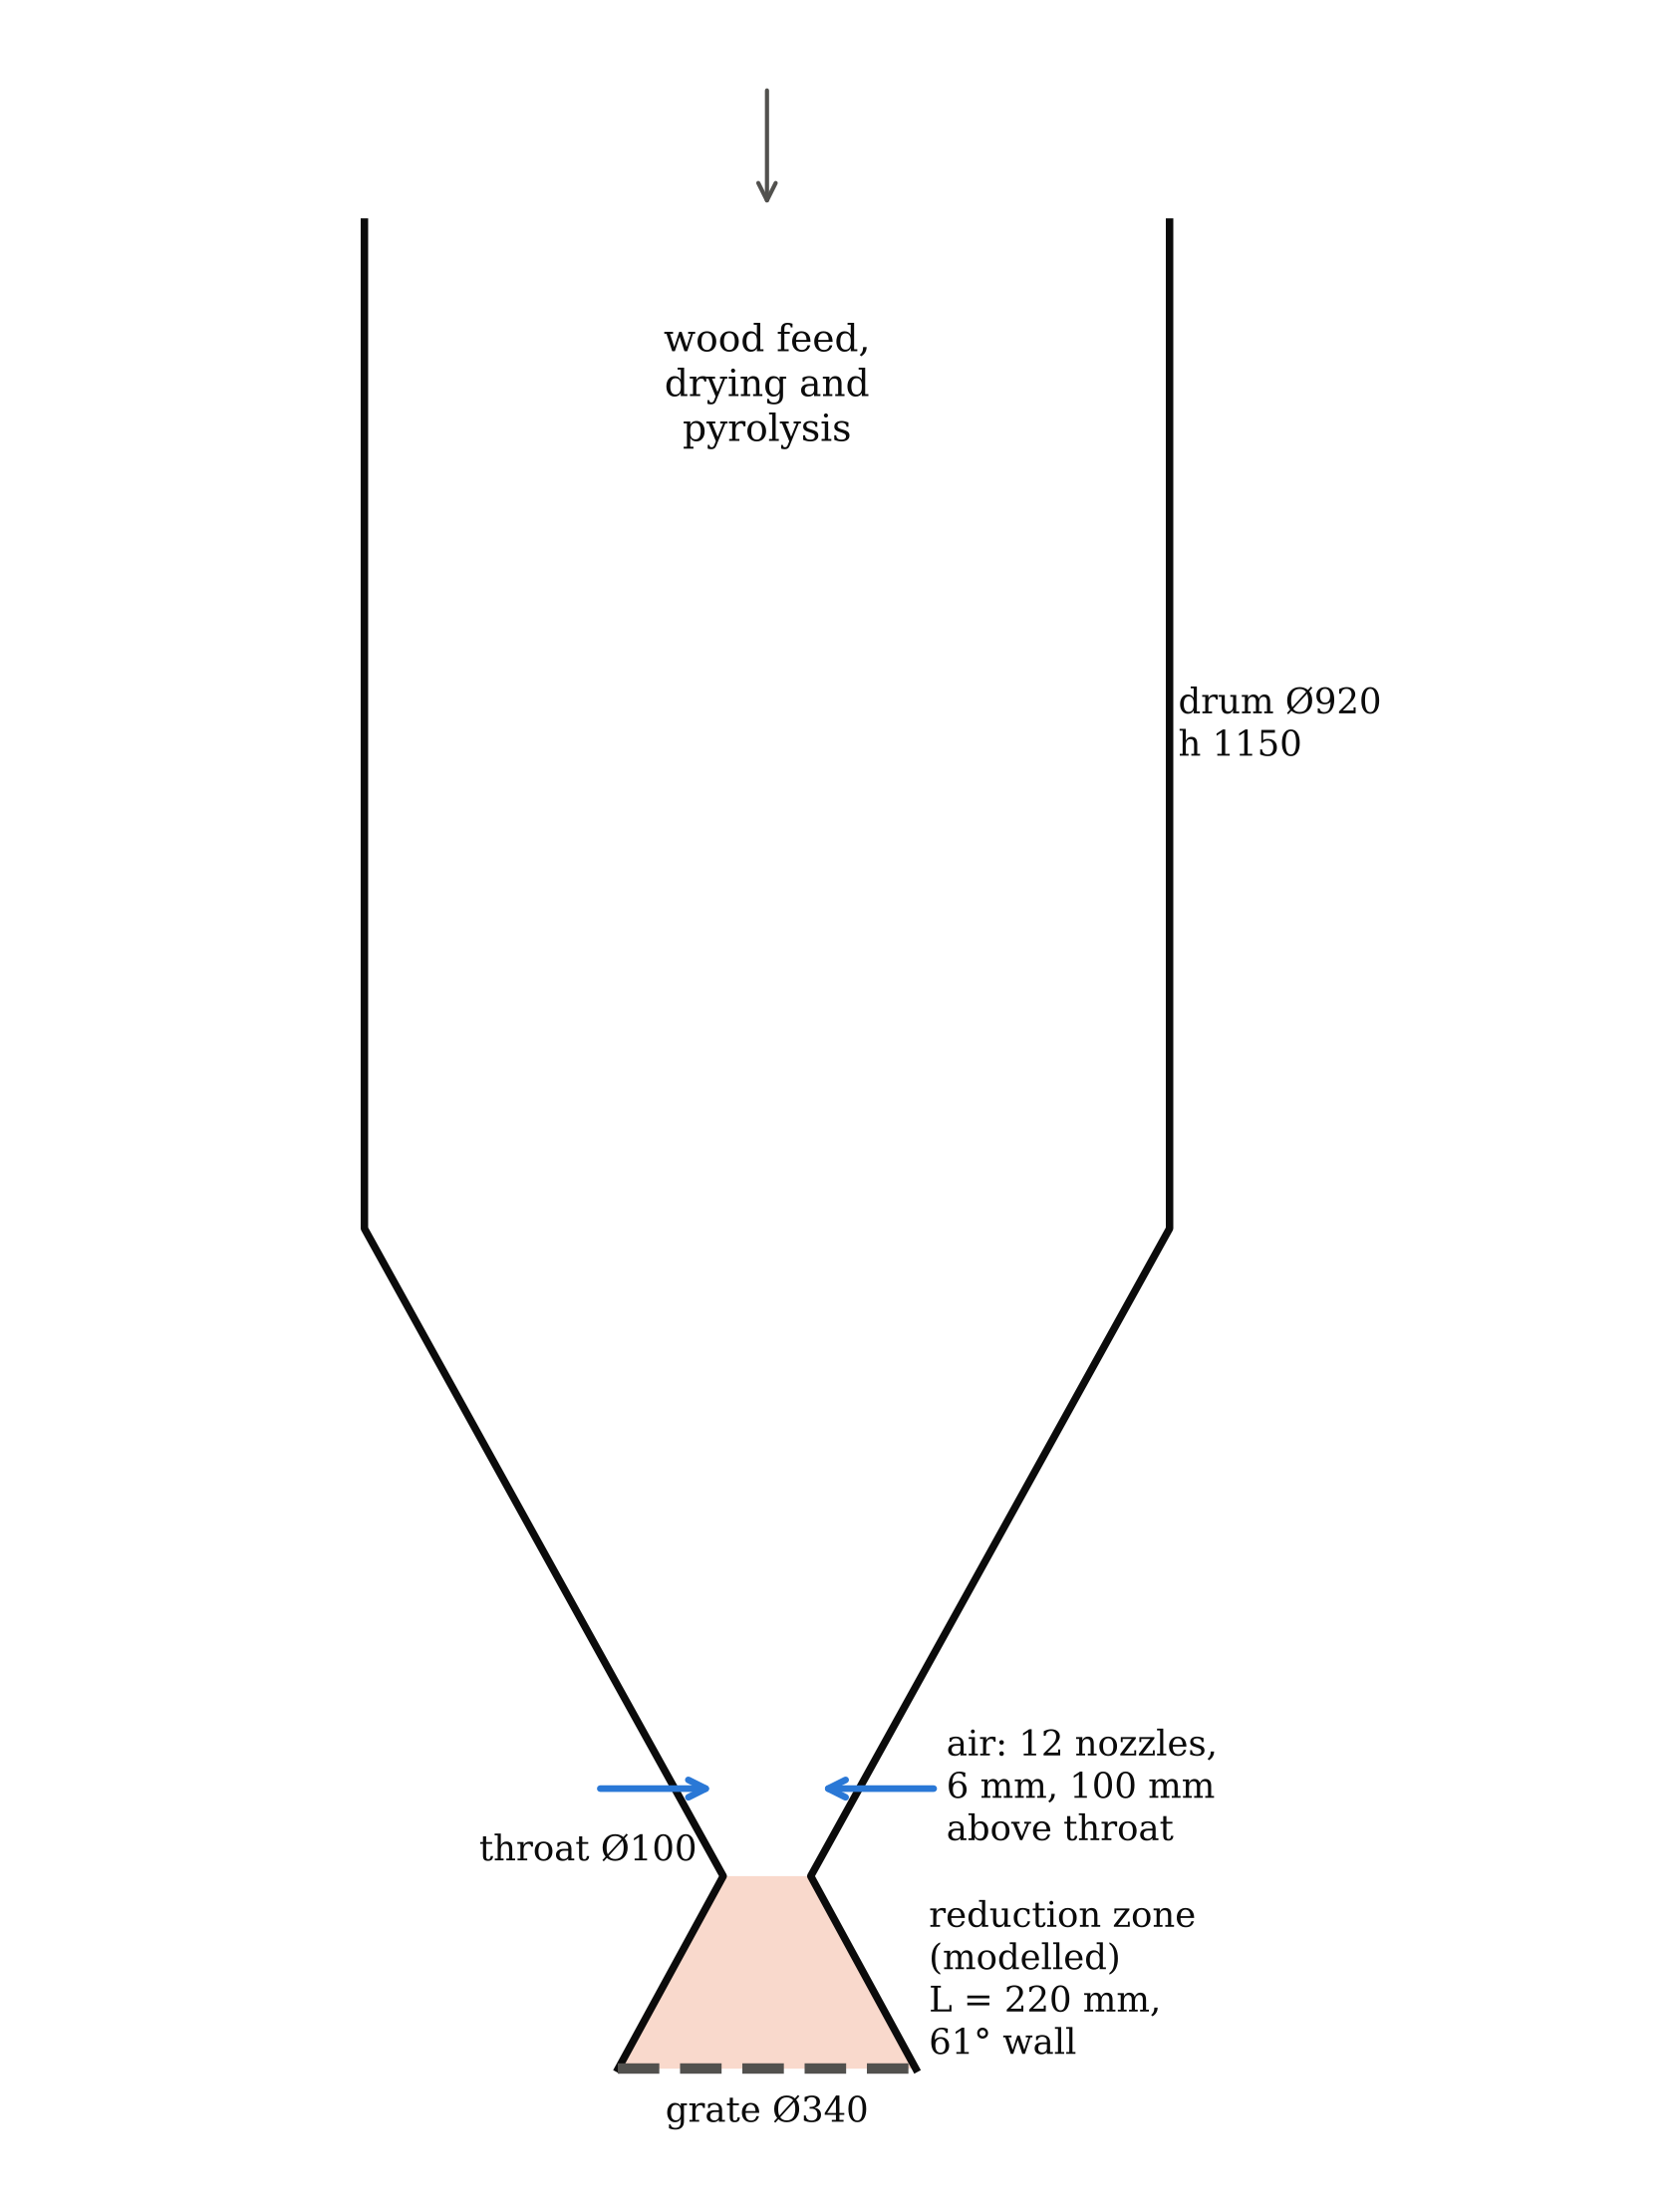
\includegraphics[width=0.48\textwidth]{fig00_geometry.png}
\caption{Geometry of the NERD gasifier as modelled (dimensions from Jayah et al.\ Fig.~3). Only the 220\,mm conical reduction zone is resolved spatially; the zones above the throat are represented by the throat sub-model.}
\label{fig:geom}
\end{figure}

\begin{table}[H]\centering\small
\caption{Geometry and operating data taken from Jayah et al.\ (2003), with assumptions marked.}
\label{tab:op}
\begin{tabularx}{\textwidth}{lXl}
\toprule
Item & Value & Source\\
\midrule
Rating & 80\,kW$_\text{th}$ & Section 4\\
Upper drum & 0.92\,m diameter, 1.15\,m long & Section 4\\
Air inlet & 12 nozzles, 6\,mm, 100\,mm above throat & Section 4\\
Throat & 100\,mm diameter, high-alumina castable & Section 4\\
Reduction zone & 220\,mm long, wall at 61$^\circ$ from horizontal, 340\,mm at the grate & Section 4, Fig.~3\\
Insulation & none (two steel skins with an air gap) & Section 4\\
Measured heat loss & 12.8\,\% of input energy & Section 8.4\\
Chip size & 3.3, 4.4, 5.5\,cm (runs); 2.5\,cm (Jayah Table~5) & Jayah Tables~3, 5\\
Moisture & 12.5--18.5\,\% d.b. & Jayah Table~3\\
Air--fuel ratio & 1.86--2.37 kg air/kg dry wood & Jayah Table~3\\
Dry wood feed rate & 18.6\,kg/h for every run (\emph{assumption}; only Jayah Table~4 gives a feed rate) & Jayah Table~4\\
Air temperature, pressure & 300\,K, 1\,atm (\emph{assumption}) & ---\\
Bed voidage & 0.48 (\emph{assumption}) & ---\\
Char particle density & 250\,kg/m$^3$ (\emph{assumption}) & ---\\
\bottomrule
\end{tabularx}
\end{table}

With the stoichiometric air requirement of \RAFRstoich\,kg/kg (calculated from Jayah Table~2), the air--fuel ratios correspond to equivalence ratios of \RERcal\ (AFR 1.86) to 0.38 (AFR 2.37); the reference case (AFR 2.20) has ER = \RERref.

%=====================================================================
\section{Feedstock and gasification chemistry}
\begin{figure}[H]\centering
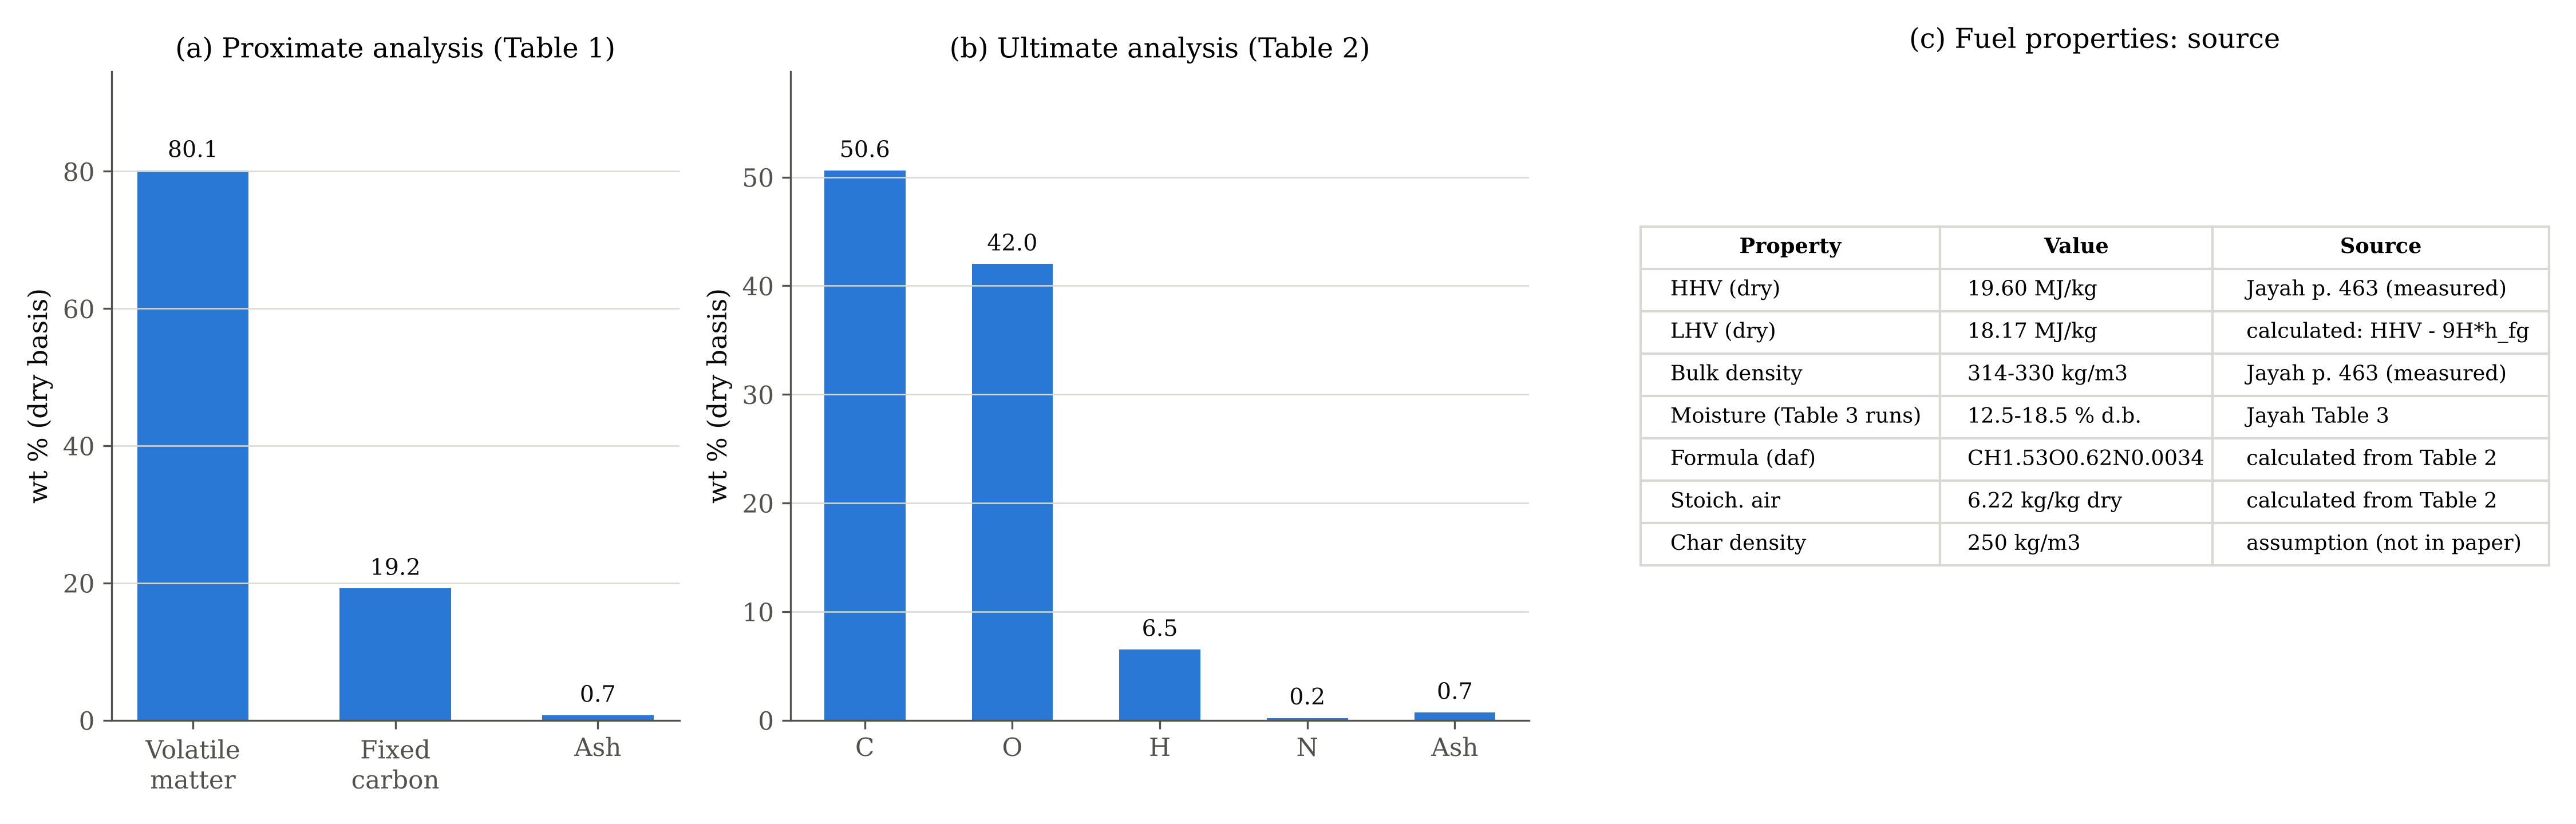
\includegraphics[width=\textwidth]{fig01_feedstock_composition.png}
\caption{Rubber wood analyses (Jayah et al.\ Tables 1--2) and derived properties, with sources.}
\end{figure}
The dry-ash-free formula is \RFormula\ and the dry LHV is \RLHVwood\,MJ/kg ($\text{LHV}=\text{HHV}-9\,w_H\,h_{fg}$).

The reduction zone is governed by:
\begin{align}
\text{C} + \text{CO}_2 &\rightleftharpoons 2\,\text{CO} & \Delta H_{298} &= +172.5~\text{kJ/mol} \quad\text{(Boudouard)}\\
\text{C} + \text{H}_2\text{O} &\rightleftharpoons \text{CO} + \text{H}_2 & \Delta H_{298} &= +131.3~\text{kJ/mol} \quad\text{(water-gas)}\\
\text{C} + 2\,\text{H}_2 &\rightleftharpoons \text{CH}_4 & \Delta H_{298} &= -74.8~\text{kJ/mol} \quad\text{(methanation)}\\
\text{CO} + \text{H}_2\text{O} &\rightleftharpoons \text{CO}_2 + \text{H}_2 & \Delta H_{298} &= -41.2~\text{kJ/mol} \quad\text{(water-gas shift)}
\end{align}
The first two consume char and heat; they set how far conversion proceeds before the bed cools. Reaction enthalpies are evaluated at the local temperature from the species heat capacities (\texttt{src/thermo.py}).

%=====================================================================
\section{Mathematical model}
\subsection{Assumptions}
\begin{enumerate}
\item Steady state, atmospheric pressure, ideal gas.
\item Above the throat, all air oxygen is consumed by the volatiles. Char (the fixed carbon, 19.2\,\% of dry wood) enters the reduction zone unreacted, as pure carbon.
\item CH$_4$ is imposed at 1.2\,\% of the dry gas leaving the throat, as Jayah et al.\ did (they set predicted methane equal to measured). CH$_4$ is therefore not a prediction.
\item Gas and char have separate temperatures ($T_g$, $T_s$). The char enters 50\,K below the gas (\emph{assumption}).
\item Particles are spheres that shrink as they react; bed voidage is constant.
\item Wall heat loss is $U\,P(z)\,(T_g-T_\infty)$, with $P$ the local wall perimeter.
\end{enumerate}

\subsection{Throat sub-model}
The volatile C, H and O, the moisture and the air are distributed among CO, CO$_2$, H$_2$, H$_2$O, CH$_4$ and N$_2$ by element balances plus water-gas-shift equilibrium. An enthalpy balance on the drying/pyrolysis/flaming zone,
\begin{equation}
\dot m_\text{wood}\,\Delta h_{f,\text{wood}} + \dot n_\text{H$_2$O(l)}\,\Delta h_{f,\text{H$_2$O(l)}} + \dot H_\text{air}(T_\text{air}) = \sum_i \dot n_i\big[\Delta h_{f,i} + h_i(T_\text{ad})\big] + \dot n_\text{C}\,h_\text{C}(T_\text{ad}-50\,\text{K}),
\end{equation}
gives the mixed-mean adiabatic temperature $T_\text{ad}$. The enthalpy of formation of wood is back-calculated from its HHV.

For the Jayah Fig.~5 condition $T_\text{ad}=\RTadRef$\,K. This is about 260\,K below the $\approx$1604\,K at which Jayah's own model curve starts (Jayah Fig.~5, digitised). A fully mixed balance cannot represent the hot near-stoichiometric flame zones at the nozzles. We therefore keep the paper's absolute level and take only the \emph{change} with operating conditions from the balance:
\begin{equation}
T_{g,0} = 1604\,\text{K} + \big[T_\text{ad}(\text{AFR},\,\text{MC},\,T_\text{air}) - T_\text{ad}(2.20,\,14.7\,\%,\,300\,\text{K})\big].
\label{eq:anchor}
\end{equation}
Across the nine runs this gives throat temperatures of \RRunTthroatMin--\RRunTthroatMax\,K: higher for more air, lower for wetter wood.

\subsection{One-dimensional reduction-zone model}
With $A(z)=\pi R(z)^2$, $R(z)=R_\text{th}+z\cot 61^\circ$, species molar flows $F_i$, char flow $F_C$, and volumetric rates $r_j$\,(mol\,m$^{-3}$\,s$^{-1}$):
\begin{align}
\frac{\dd F_i}{\dd z} &= A\sum_j \nu_{ij} r_j, \qquad \frac{\dd F_C}{\dd z} = -A\,(r_1+r_2+r_3),\\
\Big(\sum_i F_i c_{p,i}\Big)\frac{\dd T_g}{\dd z} &= h_{gs}a_p A\,(T_s-T_g) - A\,r_4\,\Delta H_4(T_g) - U\,P\,(T_g-T_\infty),\\
\dot m_C c_{p,C}\,\frac{\dd T_s}{\dd z} &= -h_{gs}a_p A\,(T_s-T_g) - A\sum_{j=1}^{3} r_j\,\Delta H_j(T_s),\\
\frac{\dd d_p}{\dd z} &= -\frac{2M_C}{\rho_\text{char}u_s}\,\frac{r_1+r_2+r_3}{a_p}, \qquad a_p=\frac{6(1-\varepsilon)}{d_p}, \qquad u_s=\frac{\dot m_C}{\rho_\text{char}(1-\varepsilon)A}.
\end{align}
The interphase coefficient $h_{gs}$ combines Ranz--Marshall convection, $Nu=2+0.6\,Re_p^{1/2}Pr^{1/3}$, with a radiative term $4\sigma e\,T^3$.

\subsection{Kinetics}\label{sec:kin}
The heterogeneous rates combine a surface reaction in series with external film mass transfer, driven by the distance from equilibrium:
\begin{equation}
r_j = a_p\,\frac{p_k - p_k^\text{eq}}{\dfrac{RT_s}{\eta_j A_j e^{-E_j/RT_s}} + \dfrac{RT_g}{k_{m,k}}}, \qquad
r_4 = \varepsilon\,k_4\Big(C_\text{CO}C_\text{H$_2$O}-\frac{C_\text{CO$_2$}C_\text{H$_2$}}{K_4}\Big),
\end{equation}
where $k_{m}$ comes from $Sh=2+1.1\,Re^{0.6}Sc^{1/3}$ and $k_4 = 2.78\times10^{-3}\exp(-1510/T_g)$\,m$^3$\,mol$^{-1}$\,s$^{-1}$.

The effectiveness factors $\eta_j$ lump intraparticle diffusion and the reactivity of this char. They are the calibrated quantities (Section~\ref{sec:cal}); Table~\ref{tab:params} lists all values.

The water-gas-shift expression $2.78\exp(-1510/T)$ is quoted in the literature without consistent concentration units. We read it as m$^3$\,kmol$^{-1}$\,s$^{-1}$, which gives a kinetically slow homogeneous shift. Taking it as m$^3$\,mol$^{-1}$\,s$^{-1}$ instead makes the shift effectively instantaneous and changes the calibration-run gas to CO \RWGSfastCO, H$_2$ \RWGSfastHtwo, CO$_2$ \RWGSfastCOtwo\,\%, far from the measurement (19.1, 15.5, 11.4\,\%). This choice is the most influential assumption in the model and is listed as a limitation.

\subsection{Two-dimensional axisymmetric model}
The cone is mapped to $\eta=r/R(z)\in[0,1]$ and split into \RTwoDcells\ annular finite-volume cells that follow the wall divergence. Each cell solves the same equations as the 1D model with its own cross-section; only the outermost cell loses heat through the wall. Neighbouring cells exchange species and heat by radial dispersion:
\begin{equation}
\left.\frac{\dd F_{i,k}}{\dd z}\right|_\text{disp} = \Big[2\pi r D_r\frac{\partial C_i}{\partial r}\Big]_{k-1/2}^{k+1/2},\qquad
\left.\Big(\sum F c_p\Big)_k\frac{\dd T_{g,k}}{\dd z}\right|_\text{disp} = \Big[2\pi r k_r\frac{\partial T_g}{\partial r}\Big]_{k-1/2}^{k+1/2},
\end{equation}
with packed-bed dispersion coefficients
\begin{align}
D_r &= \varepsilon D_m + \frac{u\,d_p}{Pe_m}, & Pe_m &= 10,\\
k_r &= \varepsilon k_g + \frac{4\sigma e}{2-e}\,d_p T^3 + \frac{\rho c_p\,u\,d_p}{Pe_h}, & Pe_h &= 8.
\end{align}
Boundary conditions are symmetry at the axis and an impermeable wall that loses heat at the outer cell. The inlet is radially uniform.

The system ($\RTwoDcells\times10$ states) is integrated as one stiff ODE system in $z$ (method of lines). A test confirms that with very strong radial mixing the 2D model collapses onto the 1D model. The model resolves radial heat and mass dispersion only: it has no velocity profile, no wall channelling, no nozzle jets, and is not CFD.

\subsection{Calibration}\label{sec:cal}
Three parameters were calibrated (\texttt{src/calibration.py}); none of the validation data were used.
\begin{enumerate}
\item The wall coefficient $U=\RUwall$\,W\,m$^{-2}$\,K$^{-1}$ makes the 22\,cm hearth lose 12.8\,\% of the feed's HHV input, the loss Jayah et al.\ measured. Jayah et al.\ themselves specify heat loss as a percentage of input energy in their gasification-zone model (their Fig.~9). The value is large for a physical wall coefficient. It should be read as an effective coefficient that assigns all of the measured loss to the uninsulated hearth.
\item The effectiveness factors $\eta_\text{B}=\RetaB$ (Boudouard) and $\eta_\text{WG}=\RetaWG$ (water-gas) minimise the squared error in CO, H$_2$ and CO$_2$ for Jayah Table~5. Jayah Table~5 is the 2.5\,cm calibration run, which the paper identifies as Run~7, so Run~7's moisture (14.7\,\%) and AFR (1.86) are used. Jayah Table~3 lists Run~7 with 5.5\,cm chips, an inconsistency in the paper.
\end{enumerate}

\subsection{Numerical method}
The 1D equations are integrated with SciPy's implicit Radau method (relative tolerance $10^{-5}$, absolute $10^{-8}$). The 2D system uses Radau with the block-tridiagonal Jacobian sparsity ($\RTwoDnz$ output stations). The complete pipeline runs in about \RRuntime\,s.

%=====================================================================
\section{Verification}
\begin{itemize}
\item \textbf{Element balances:} C, H, O and N close to machine precision ($<10^{-12}$\,\%), because the stoichiometry conserves them exactly.
\item \textbf{Energy balance:} with total (formation + sensible) enthalpy flows, $\dot H(0)-\dot H(L)-\dot Q_\text{wall}$ is \REnergyResidual\,\% of the feed HHV. The residual comes from evaluating heterogeneous reaction heats at $T_s$.
\item \textbf{Automated tests (20):}
  \begin{itemize}
  \item feedstock arithmetic, thermodynamics and reaction rates;
  \item conservation;
  \item the throat temperature rising with AFR and air pre-heat and falling with moisture;
  \item all validation statistics recomputed independently;
  \item the 2D$\to$1D limit.
  \end{itemize}
  Run with \texttt{python -m pytest tests}.
\end{itemize}

%=====================================================================
\section{Results: reference case}
The reference case is the Jayah Fig.~5 condition: AFR 2.20 (ER \RERref), 2.5\,cm chips, 14.7\,\% d.b. moisture, and the 22\,cm hearth.

\begin{table}[H]\centering\small
\caption{Reference-case results at the hearth exit ($z=22$\,cm), 1D model.}
\begin{tabular}{lr}
\toprule
Throat gas temperature $T_{g,0}$ (mixed adiabatic value) & \RTthroatRef\,K (\RTadRef\,K)\\
Exit gas temperature & \RTexitRef\,K\\
Dry gas: CO / H$_2$ / CO$_2$ / CH$_4$ / N$_2$ & \RCOexitRef\ / \RHtwoExitRef\ / \RCOtwoExitRef\ / \RCHfourExitRef\ / \RNtwoExitRef\,\%\\
Gas LHV & \RLHVRef\,MJ/Nm$^3$\\
Dry gas flow (at 18.6\,kg/h dry wood) & \RFlowRef\,Nm$^3$/h\\
Conversion (cold-gas) efficiency, LHV$_\text{gas}$/HHV$_\text{wood}$ & \RCGERef\,\%\\
Char conversion & \RXcRef\,\%\\
Exit particle diameter (from 2.5\,cm) & \RdpExitRef\,cm\\
Wall heat loss & \RWallkWRef\,kW (\RWallPctRef\,\% of \RQinRef\,kW input)\\
\bottomrule
\end{tabular}
\end{table}

\subsection{Axial species distribution}
\begin{figure}[H]\centering
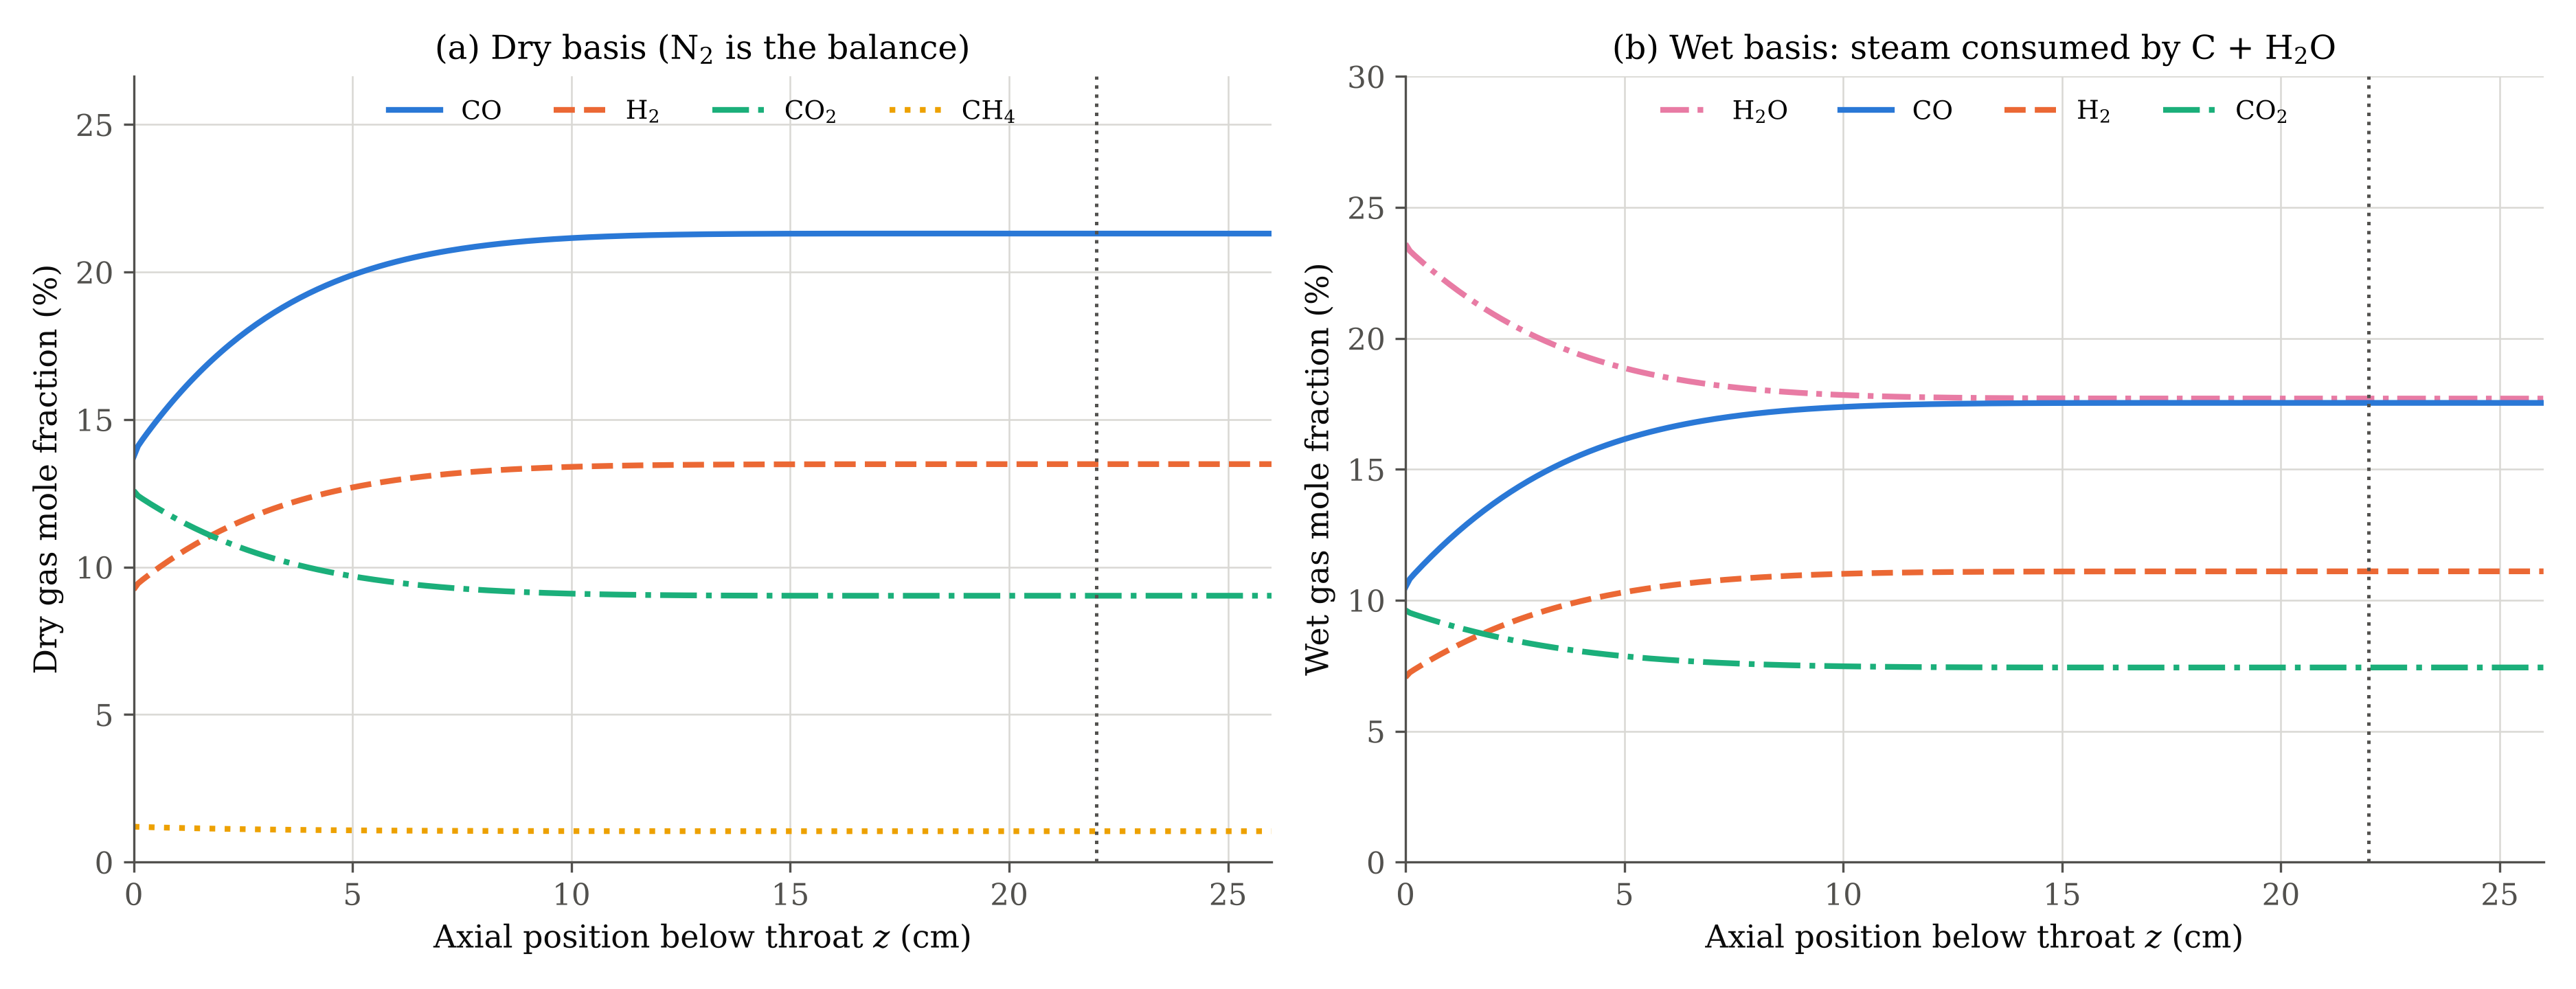
\includegraphics[width=\textwidth]{fig02_species_distributions_1d.png}
\caption{Axial species profiles in the reduction zone (reference case): (a) dry basis, (b) wet basis including steam.}
\end{figure}
CO rises from \RCOthroatRef\ to \RCOexitRef\,\% and H$_2$ from \RHtwoThroatRef\ to \RHtwoExitRef\,\%, while CO$_2$ falls from \RCOtwoThroatRef\ to \RCOtwoExitRef\,\% and steam from \RHtwoOinRef\ to \RHtwoOoutRef\,\% (wet). Almost all of the change happens in the first 8--10\,cm. Beyond that the bed is too cold (below about 1150\,K) for the char reactions to proceed, and the composition freezes.

\subsection{Char conversion}
\begin{figure}[H]\centering
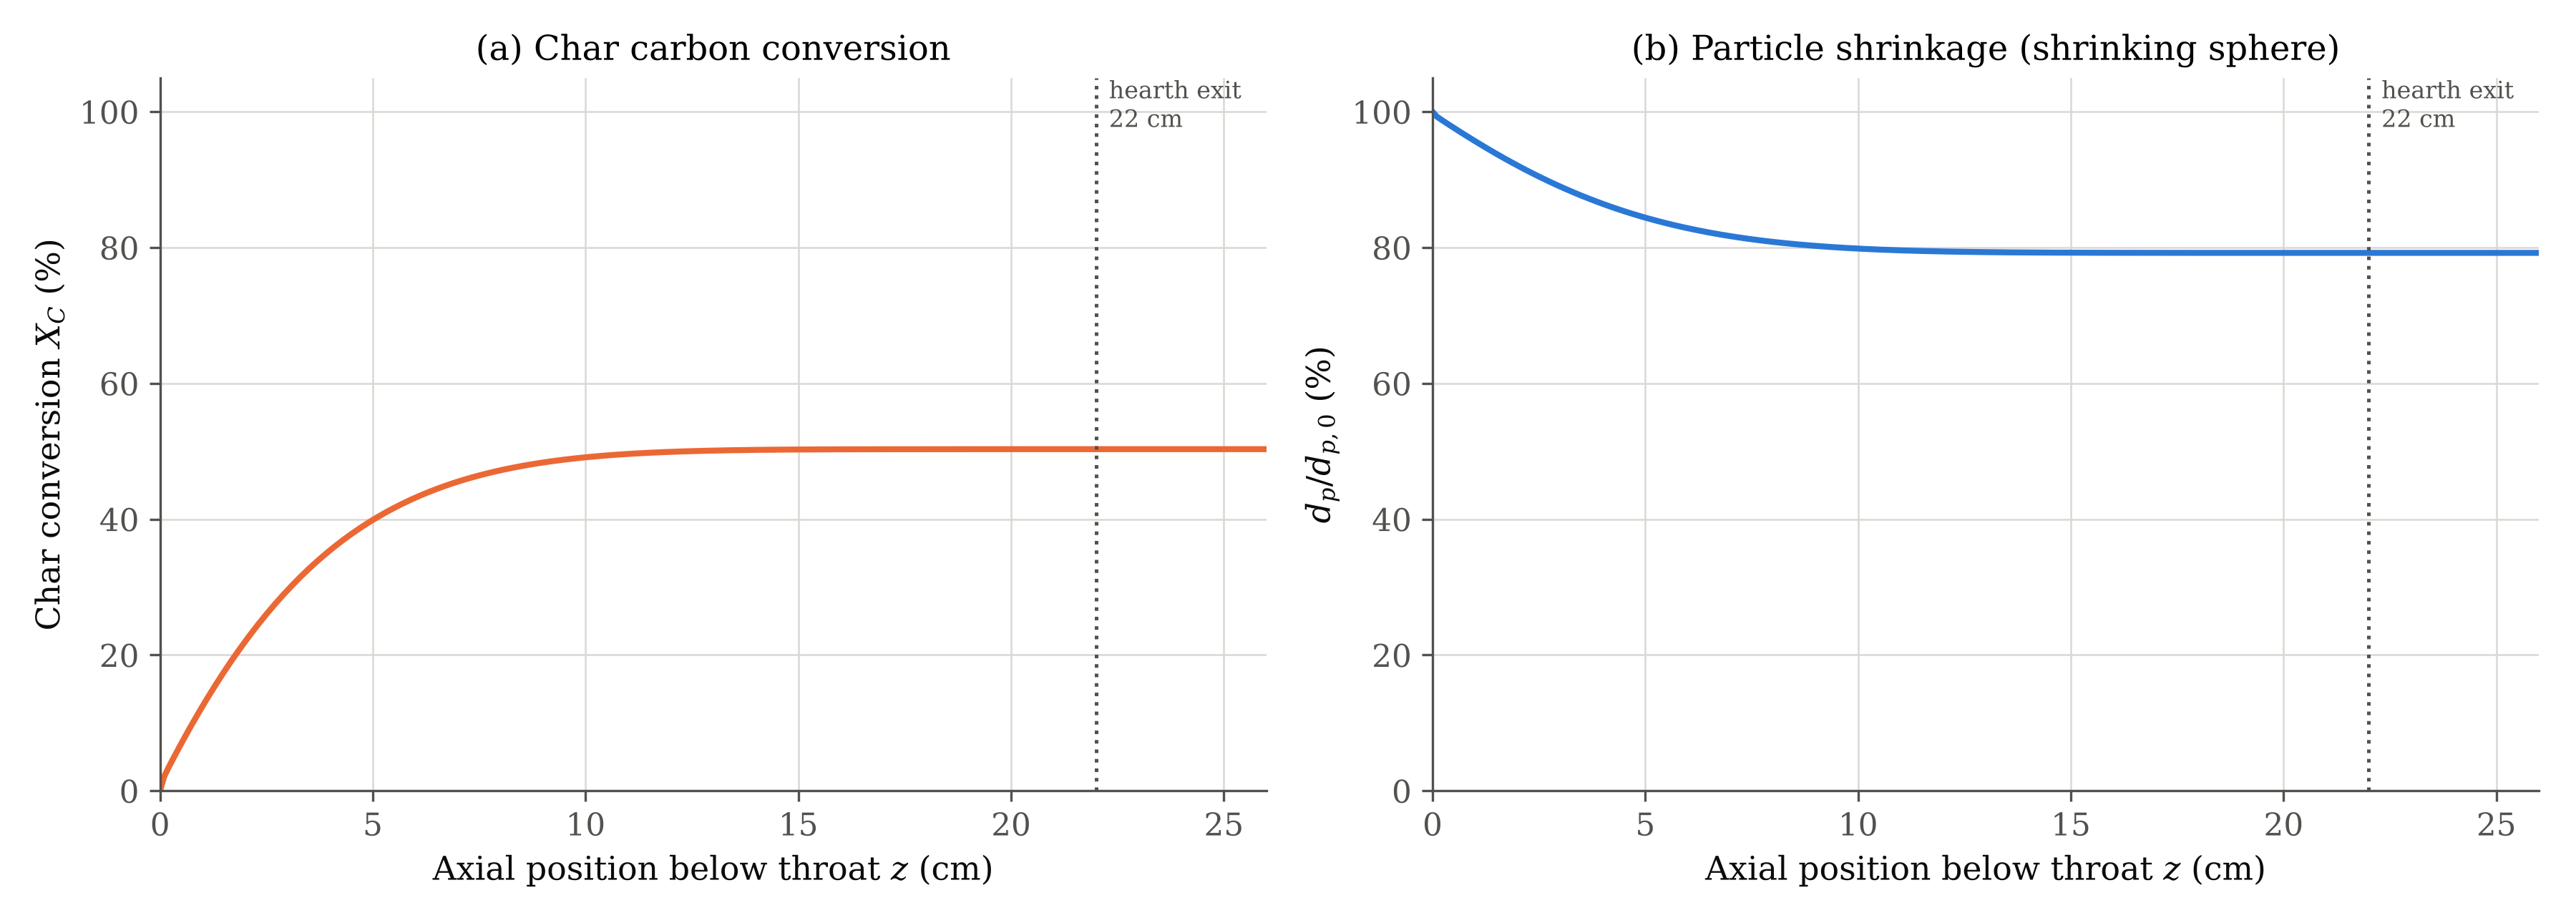
\includegraphics[width=0.95\textwidth]{fig04_char_conversion_and_shrinkage.png}
\caption{Char conversion and particle shrinkage along the bed (reference case).}
\end{figure}
Half of the final conversion is reached by $z=\RzHalfRef$\,cm, and conversion stops at \RXcRef\,\%. A quick check against Jayah's Table~4: 0.7--2.1\,kg/h of char leaves the grate, out of about 3.6\,kg/h of fixed carbon, i.e.\ 41--80\,\% conversion. The reference case lies at the lower end of that range. The calibration run (AFR 1.86) converts only \RCalXc\,\%, which is low (Section~\ref{sec:lim}).

\subsection{Temperature}
\begin{figure}[H]\centering
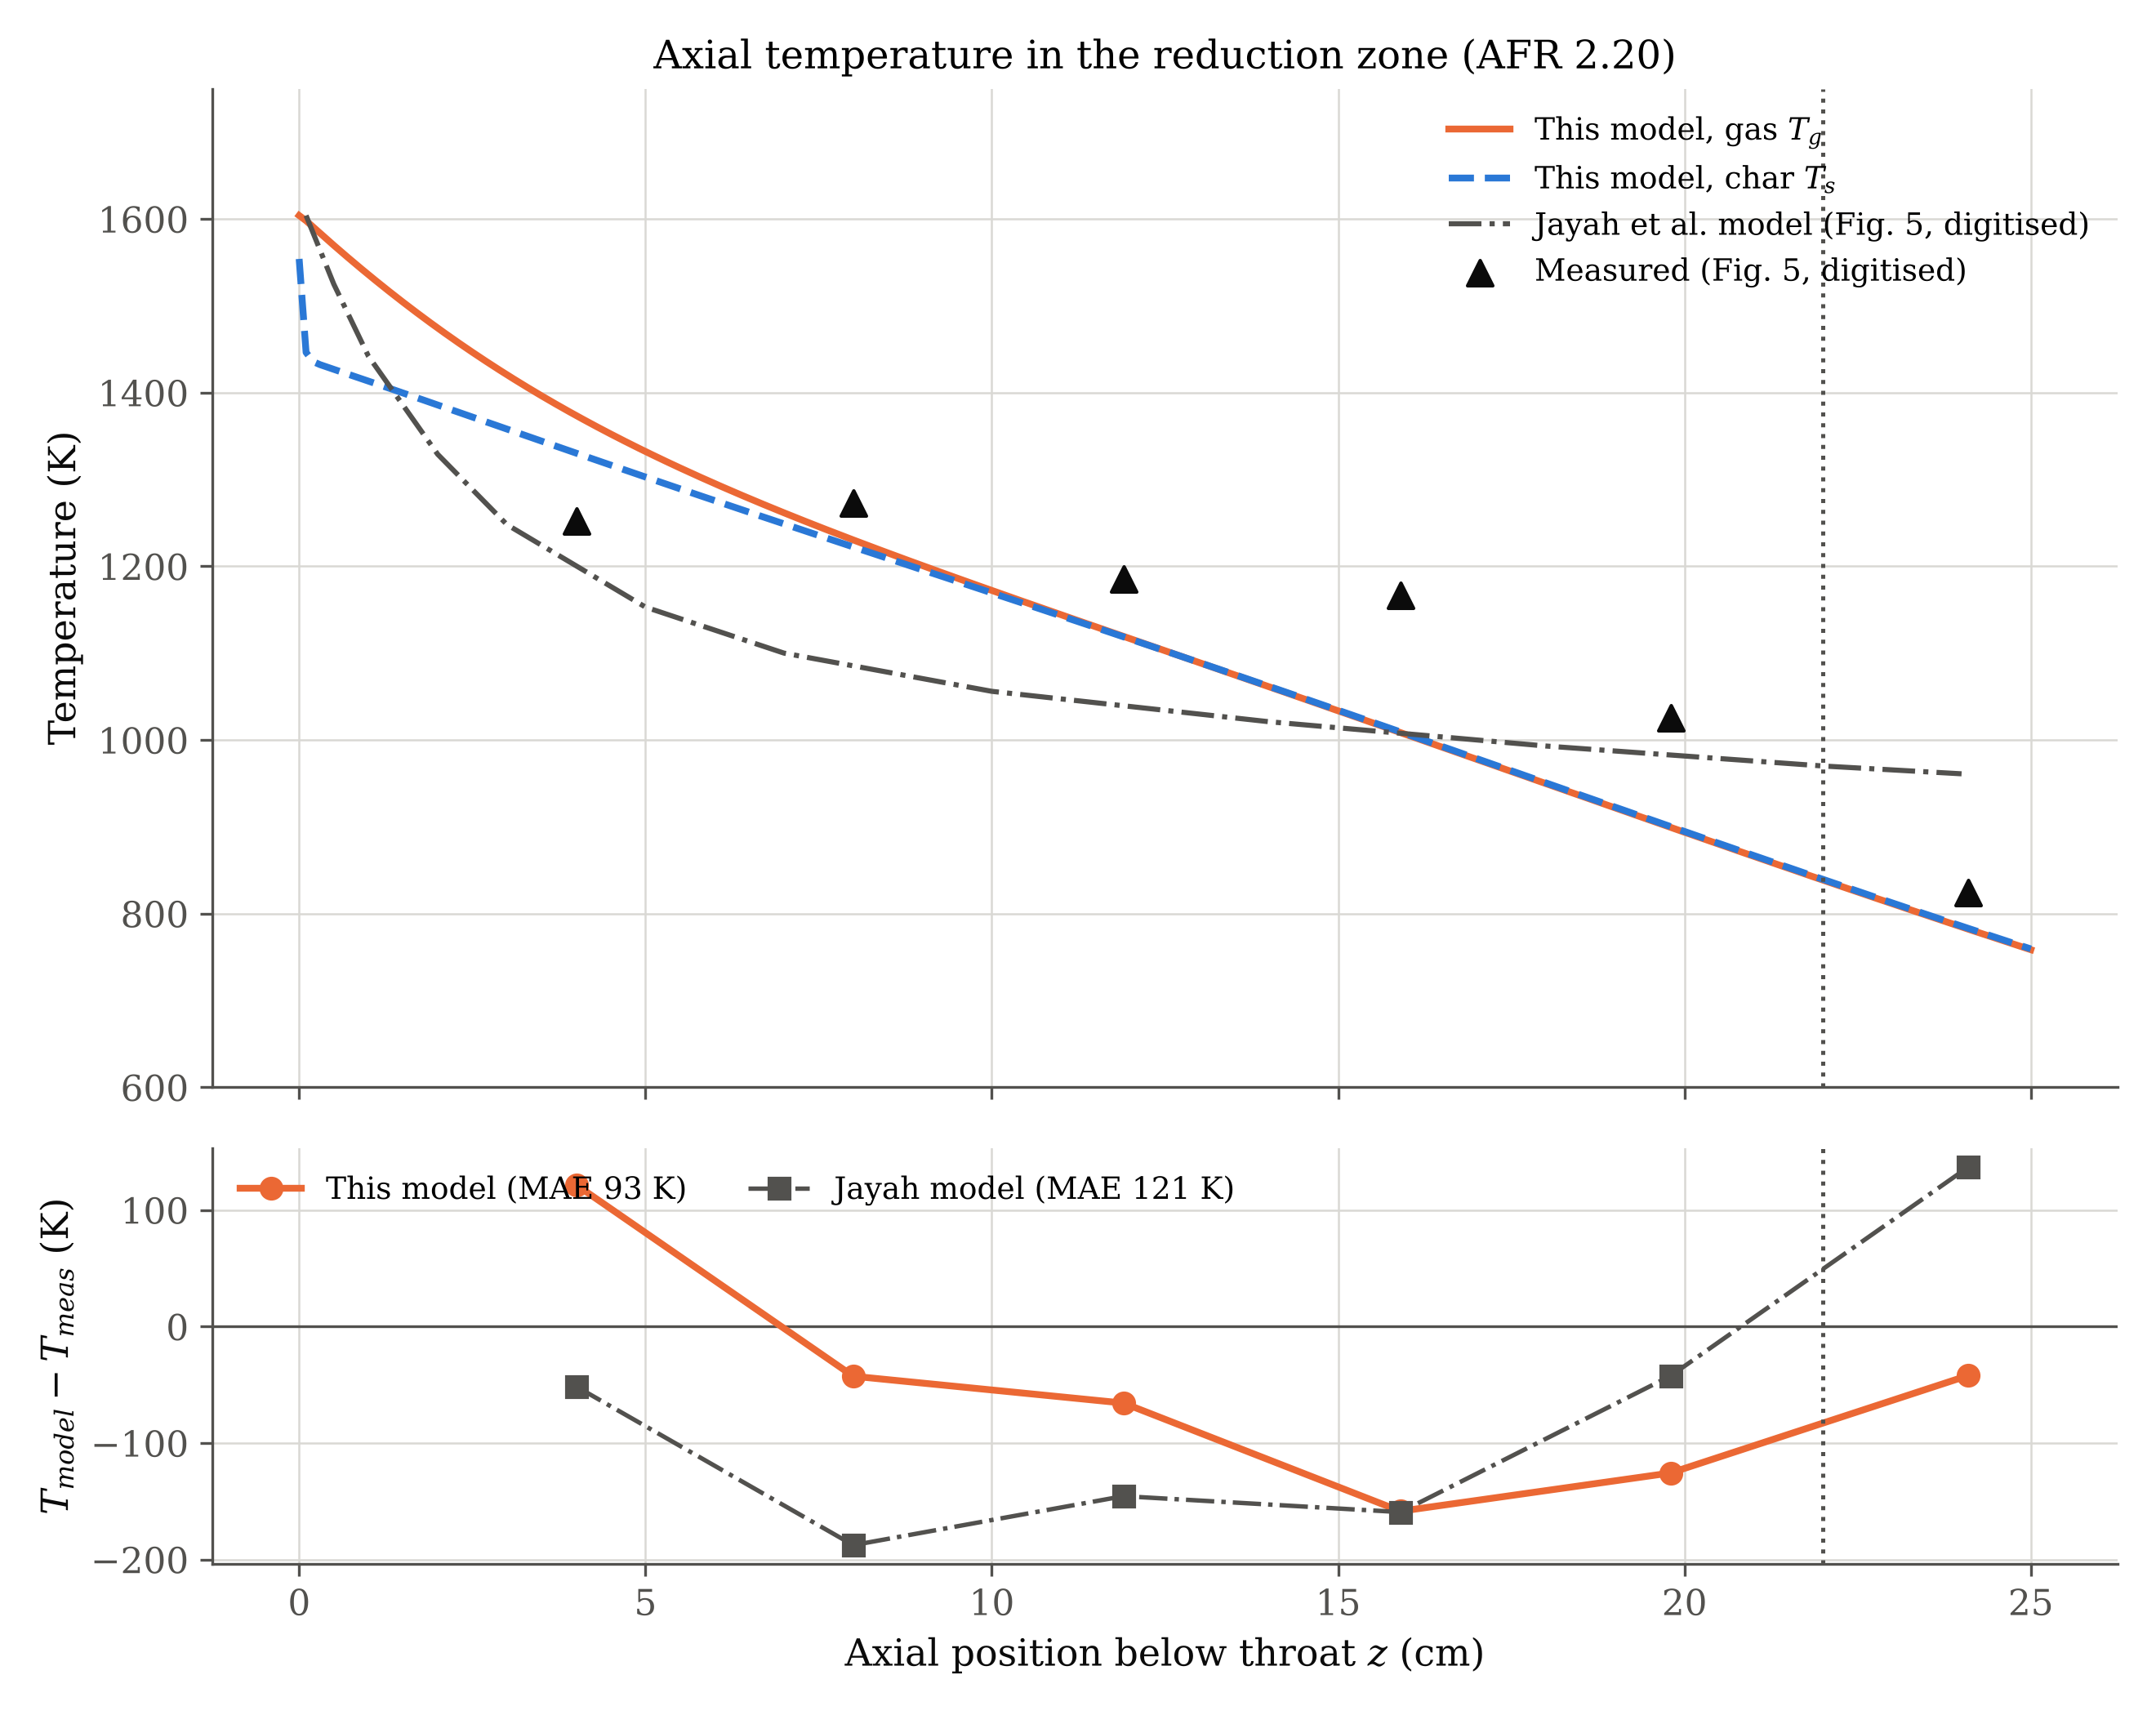
\includegraphics[width=0.8\textwidth]{fig03_temperature_profiles_1d.png}
\caption{Gas and char temperatures against the six measured points and Jayah's model curve, both digitised from Jayah Fig.~5; the lower panel shows the errors.}
\end{figure}
The gas enters at \RTthroatRef\,K and the char at \RTsZeroRef\,K. The char, with its small heat capacity flow, is cooled immediately by its own endothermic reactions, opening a gas--char gap of up to \RdTgsMax\,K. The two phases equilibrate (gap below 10\,K) by $z=\RzEquil$\,cm.

The gas cools to \RTfiveRef\,K at 5\,cm, \RTtenRef\,K at 10\,cm and \RTexitRef\,K at the exit. Of the \RSensDrop\,kW of sensible heat the gas and char lose across the hearth, \RWallShare\,\% leaves through the wall (\RWallkWRef\,kW) and \RRxnShare\,\% is absorbed by the endothermic reactions. Section~\ref{sec:val} compares these temperatures with the measurements.

\subsection{Two-dimensional species and temperature fields}
\begin{figure}[H]\centering
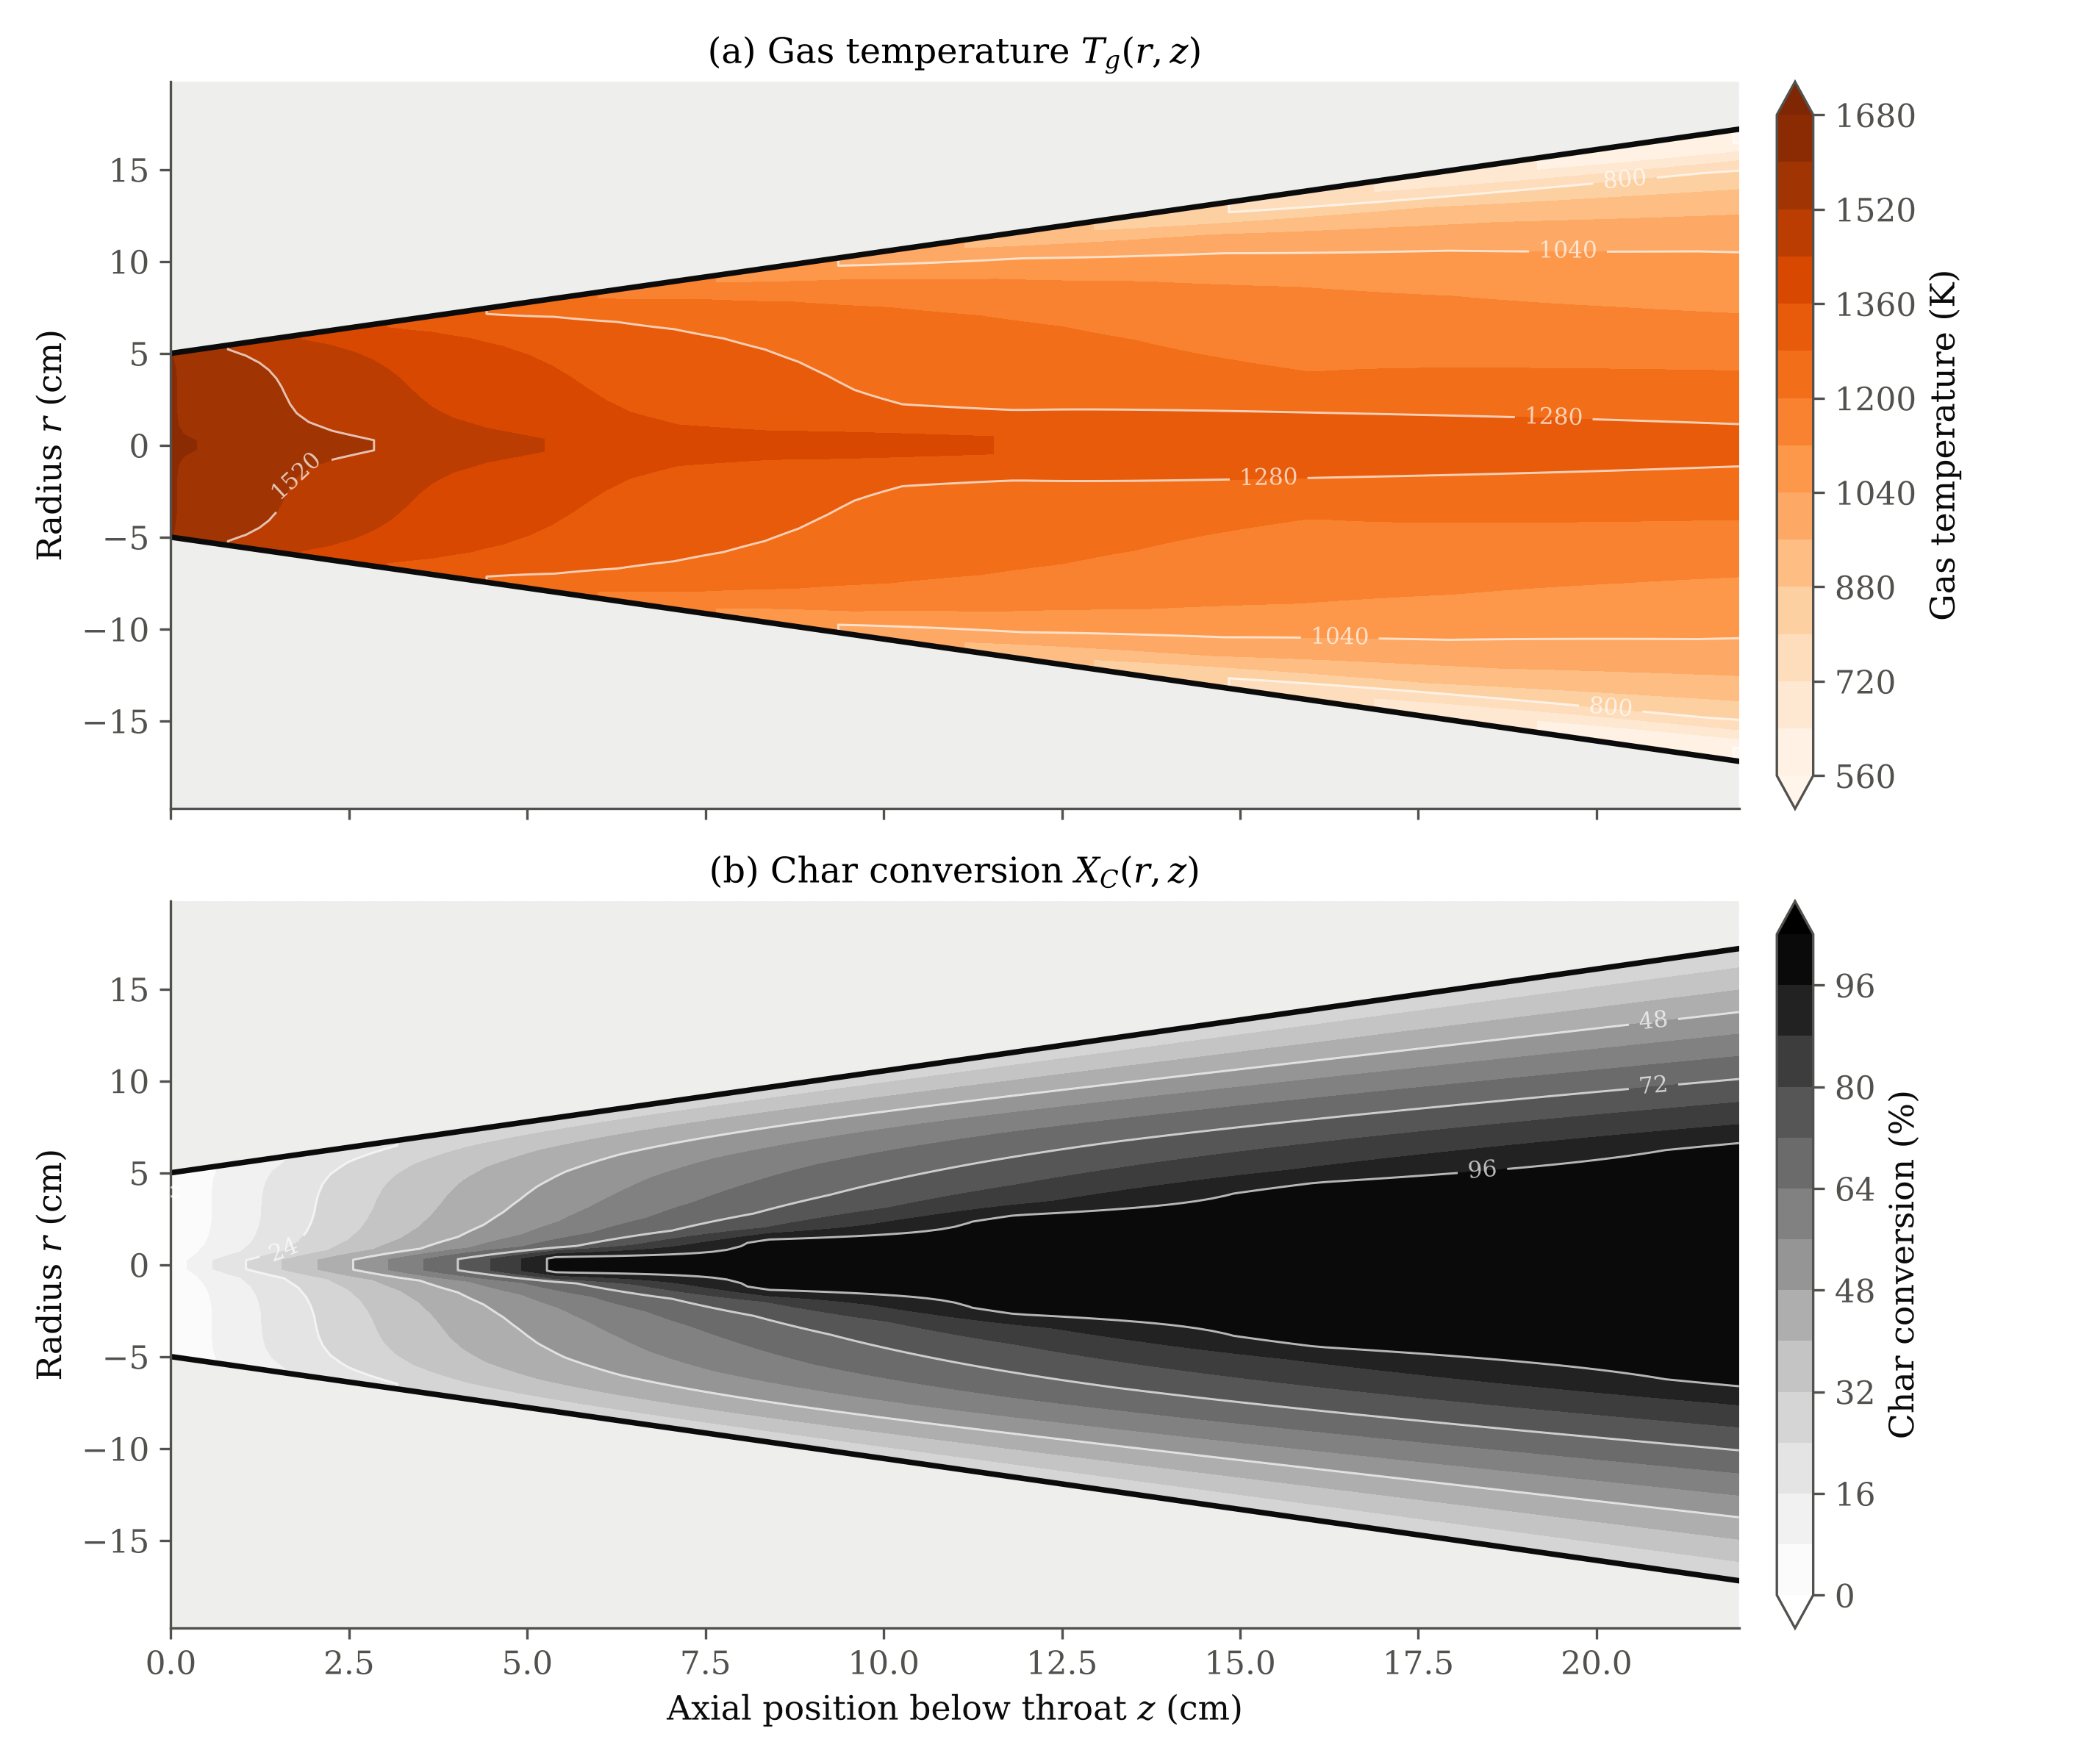
\includegraphics[width=0.82\textwidth]{fig05_temperature_contours_2d.png}
\caption{2D model: gas temperature and char conversion in the conical hearth (mirrored about the axis).}
\end{figure}
\begin{figure}[H]\centering
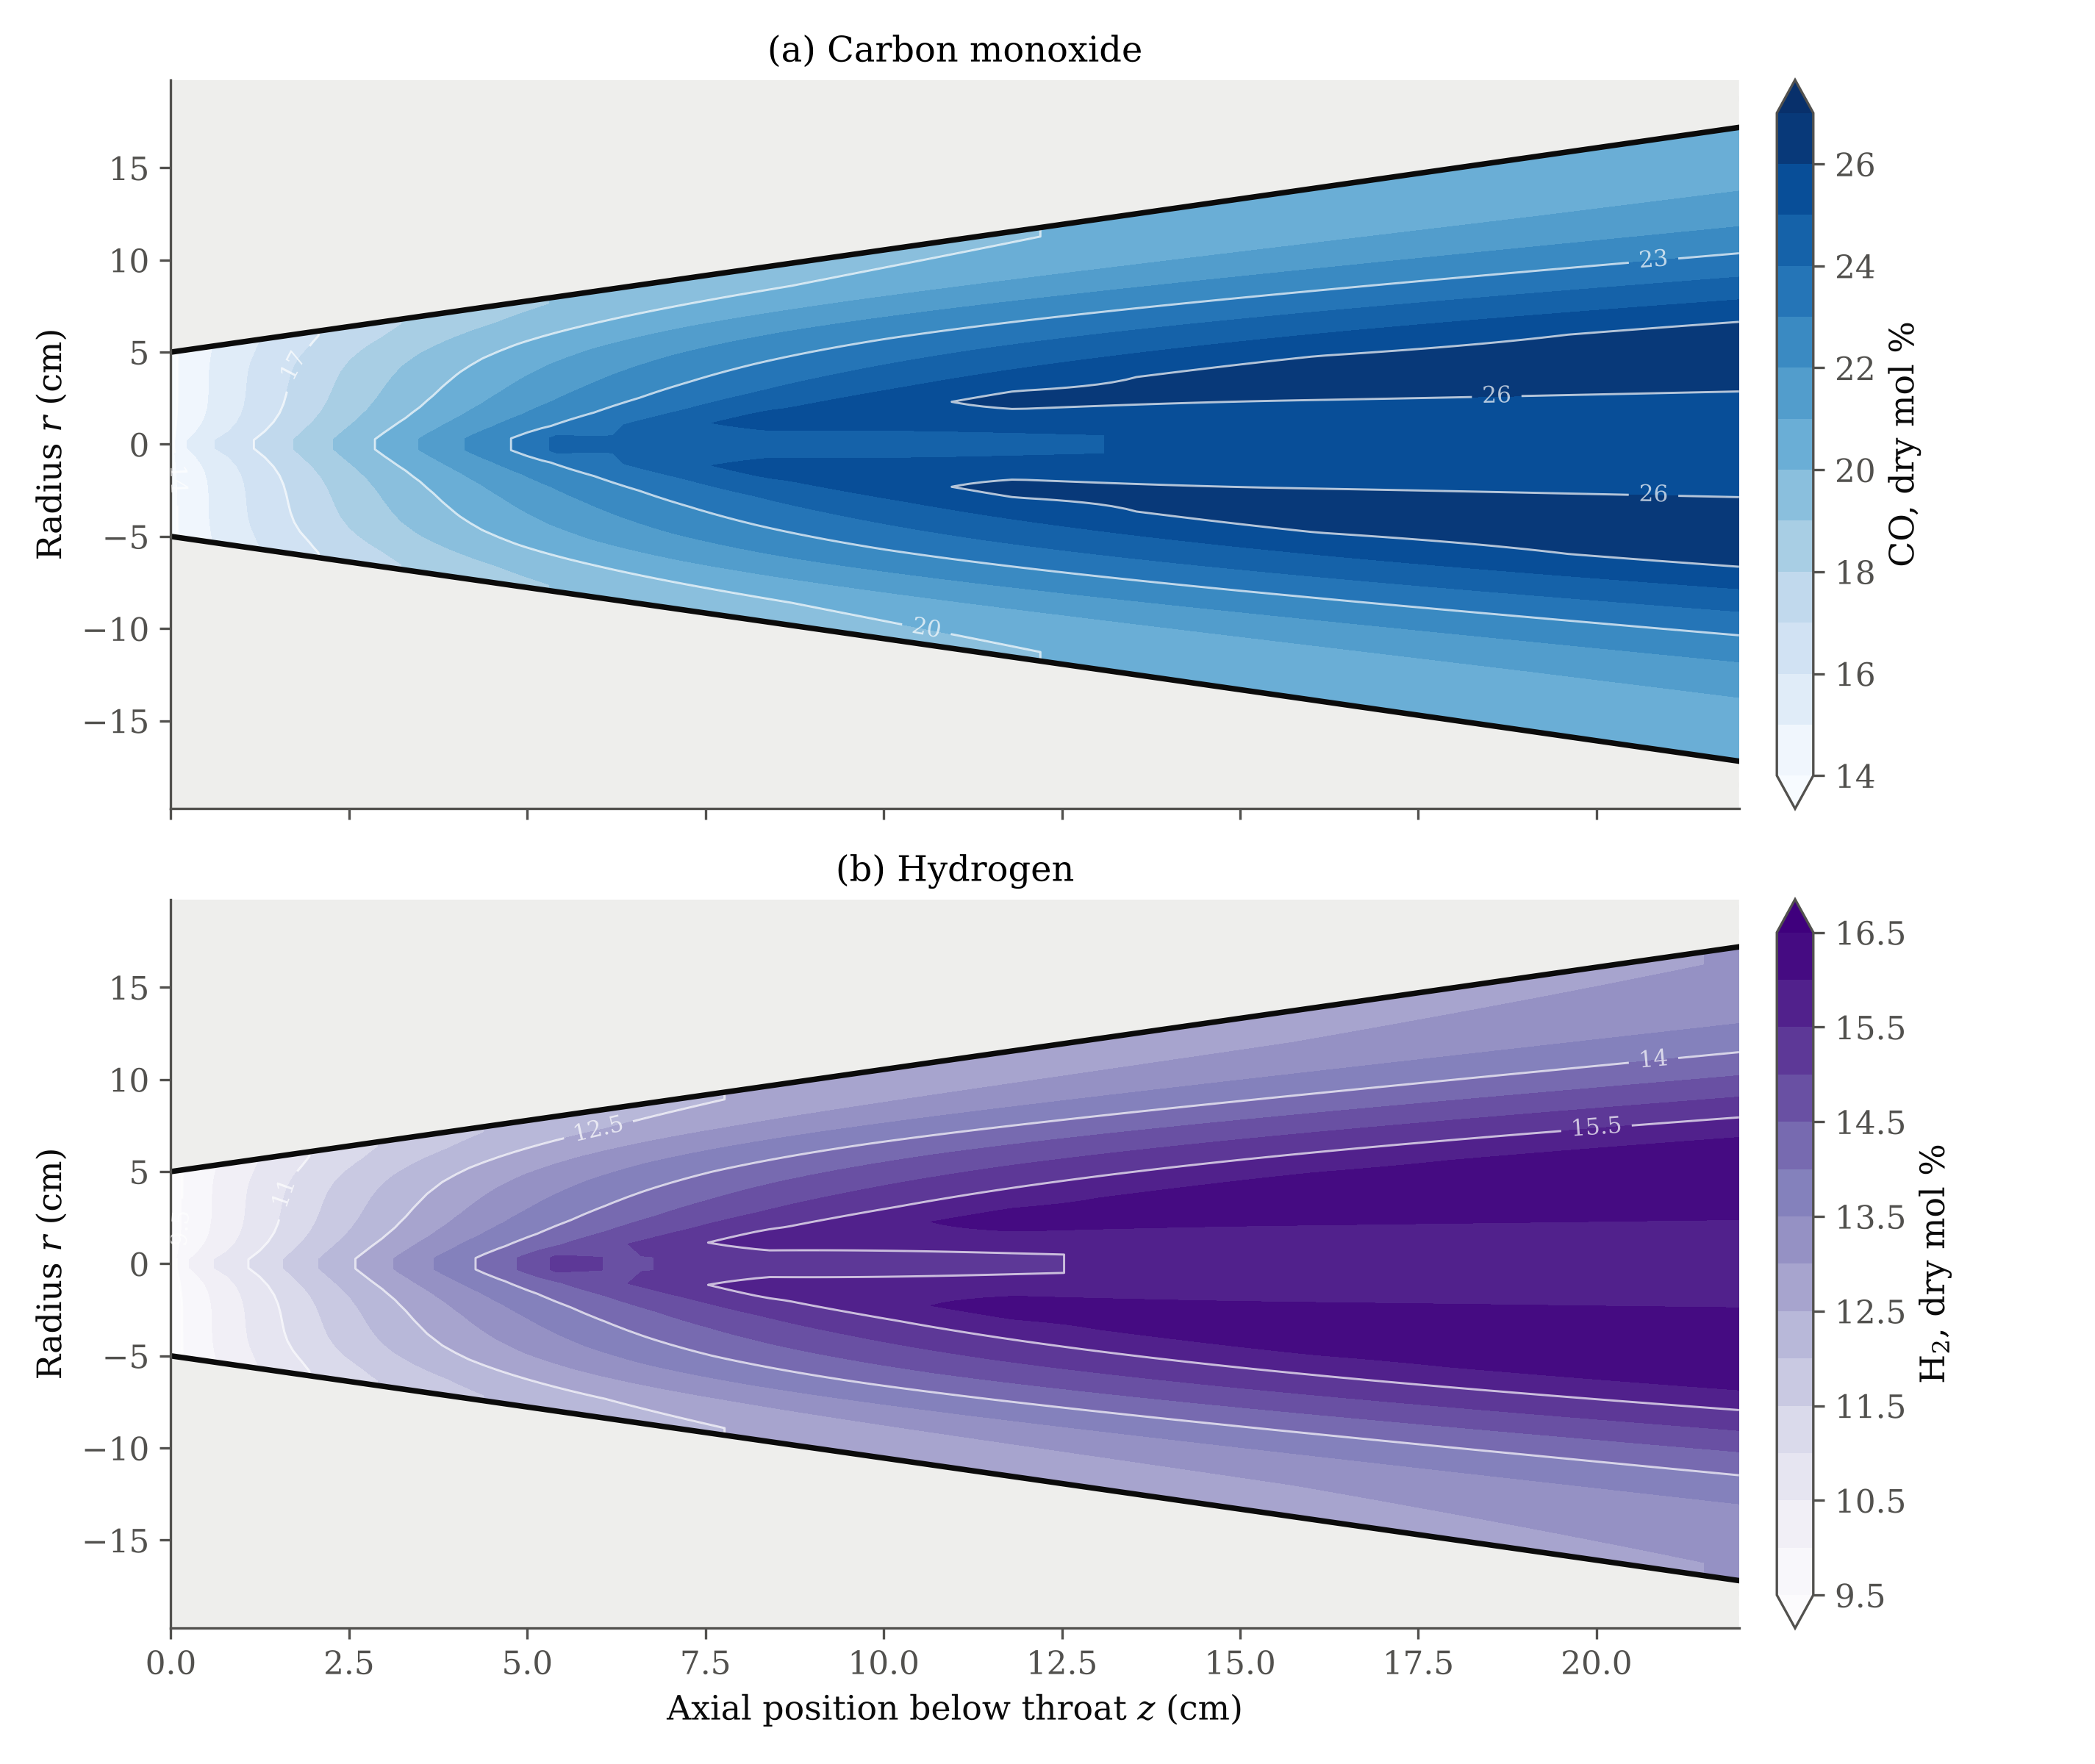
\includegraphics[width=0.82\textwidth]{fig06_species_contours_fuel_2d.png}
\caption{2D model: CO and H$_2$ (dry basis).}
\end{figure}
\begin{figure}[H]\centering
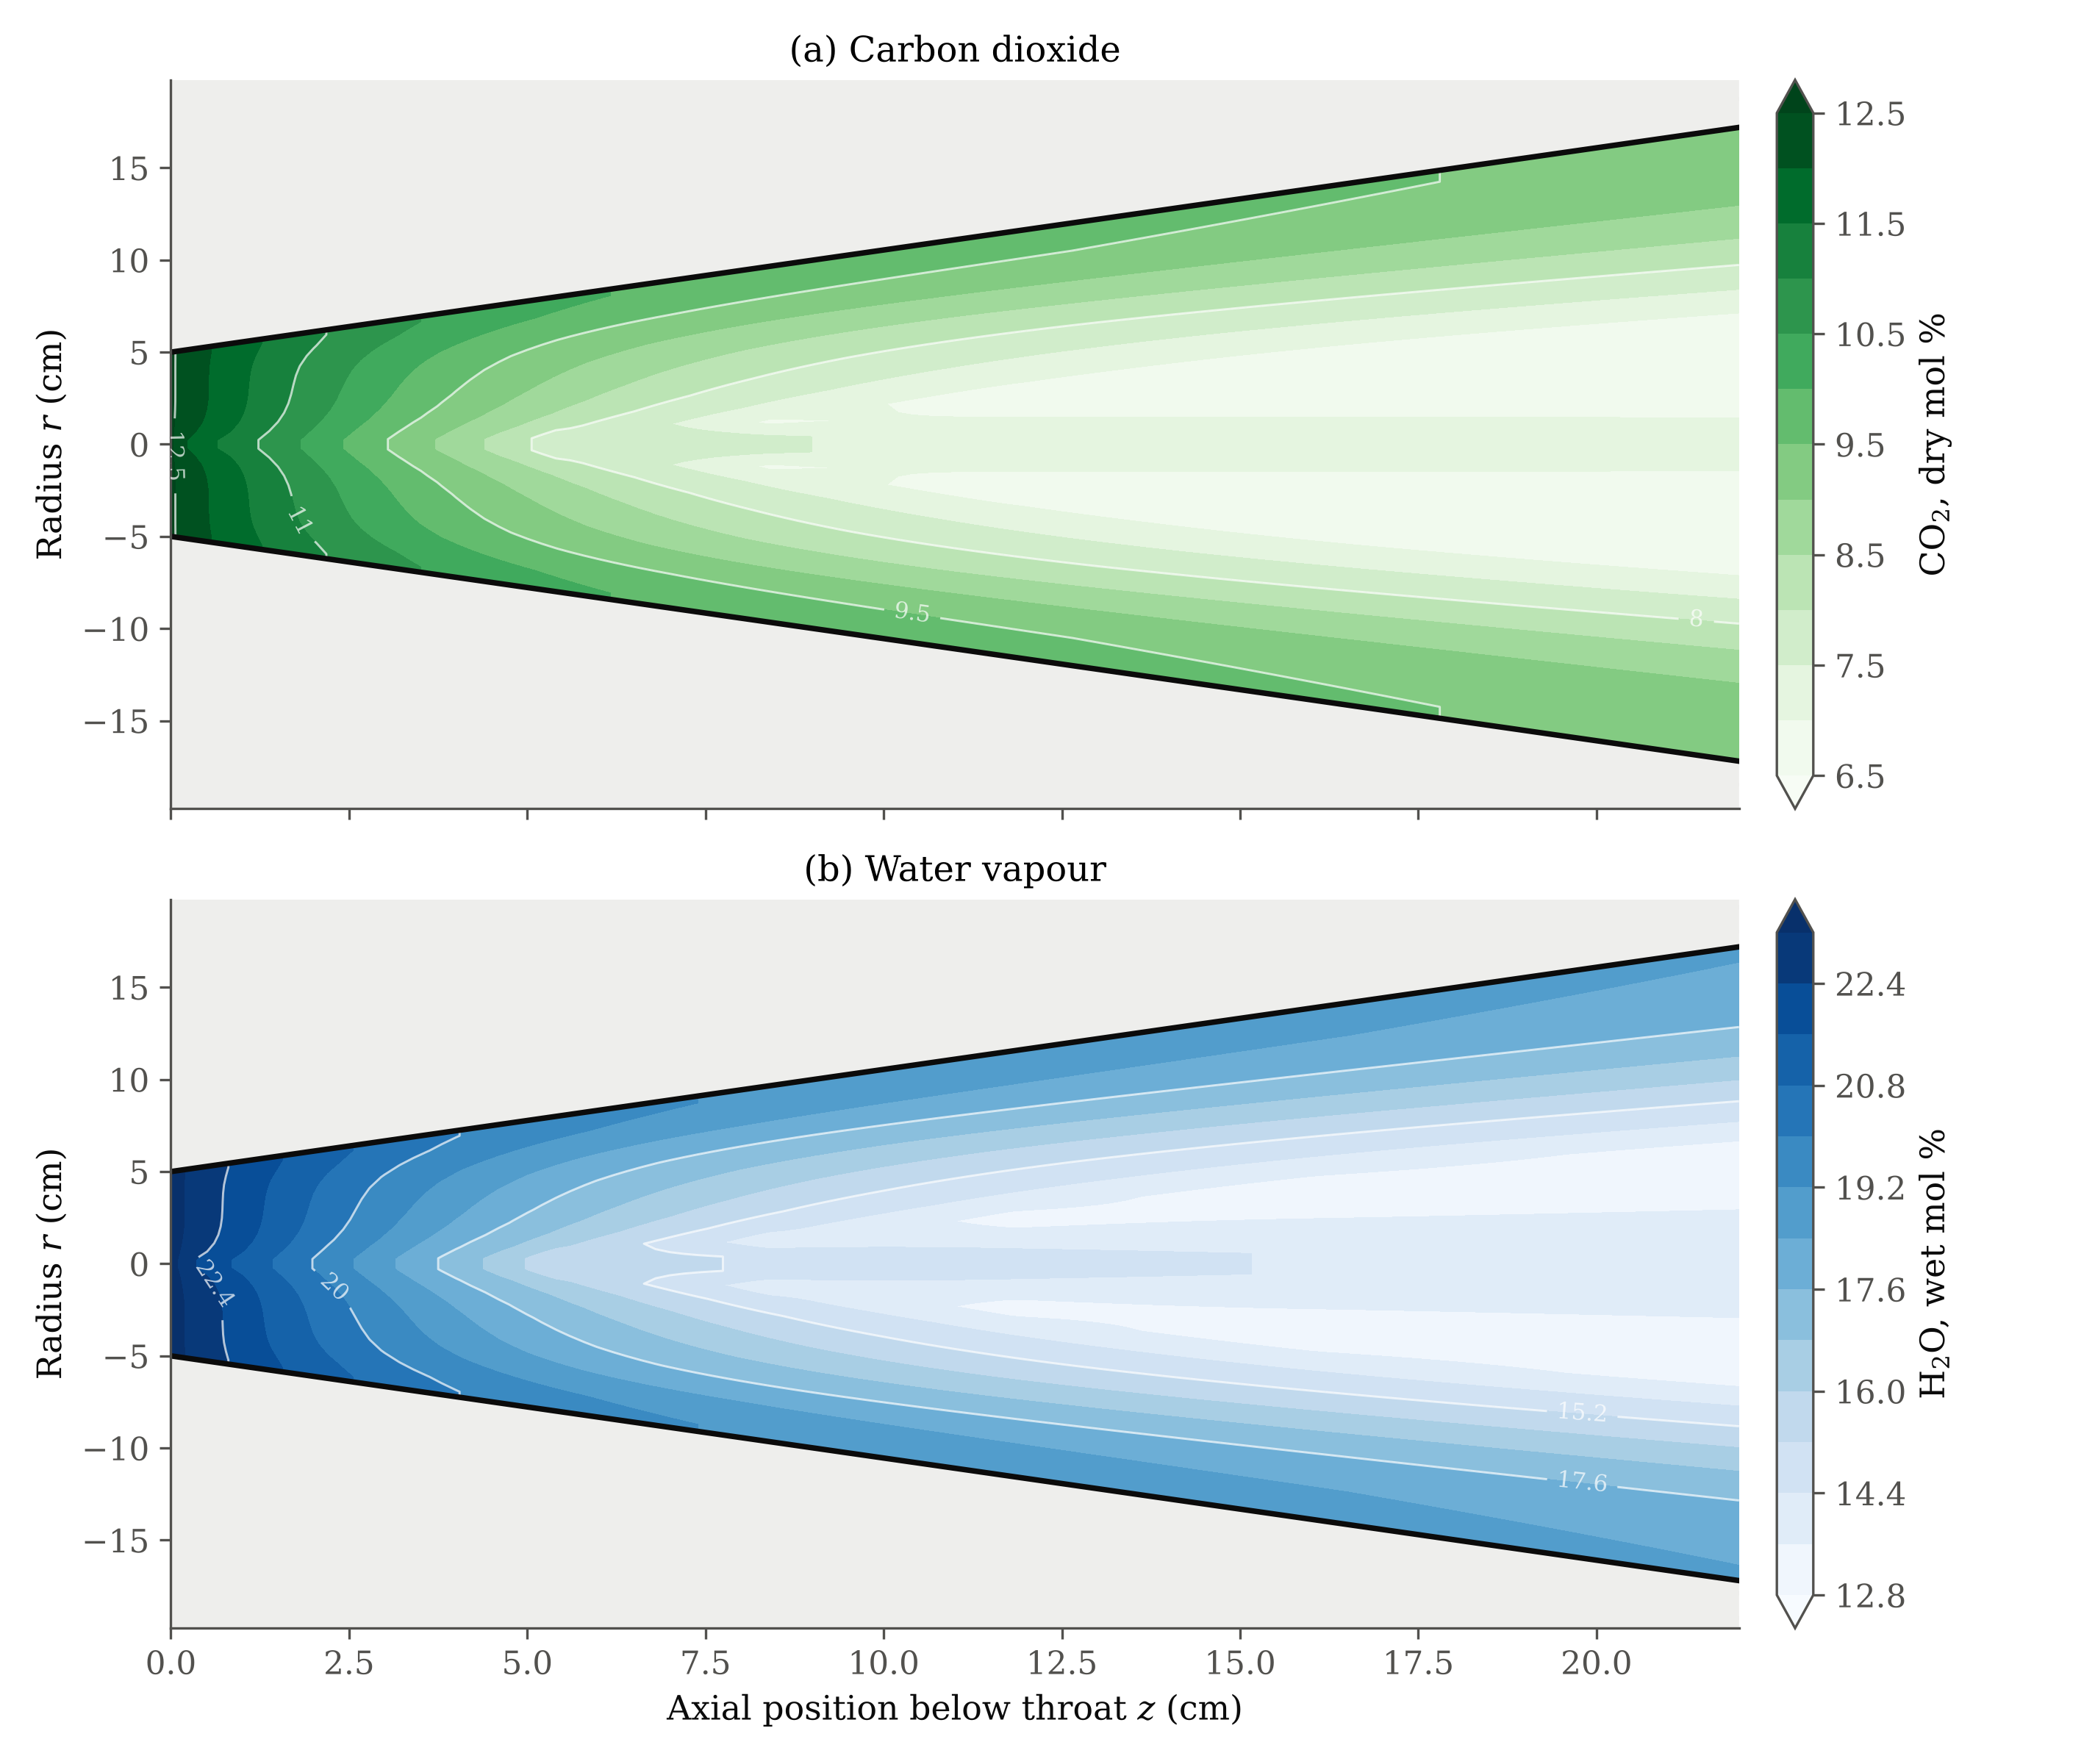
\includegraphics[width=0.82\textwidth]{fig07_species_contours_oxidants_2d.png}
\caption{2D model: CO$_2$ (dry) and H$_2$O (wet).}
\end{figure}
\begin{figure}[H]\centering
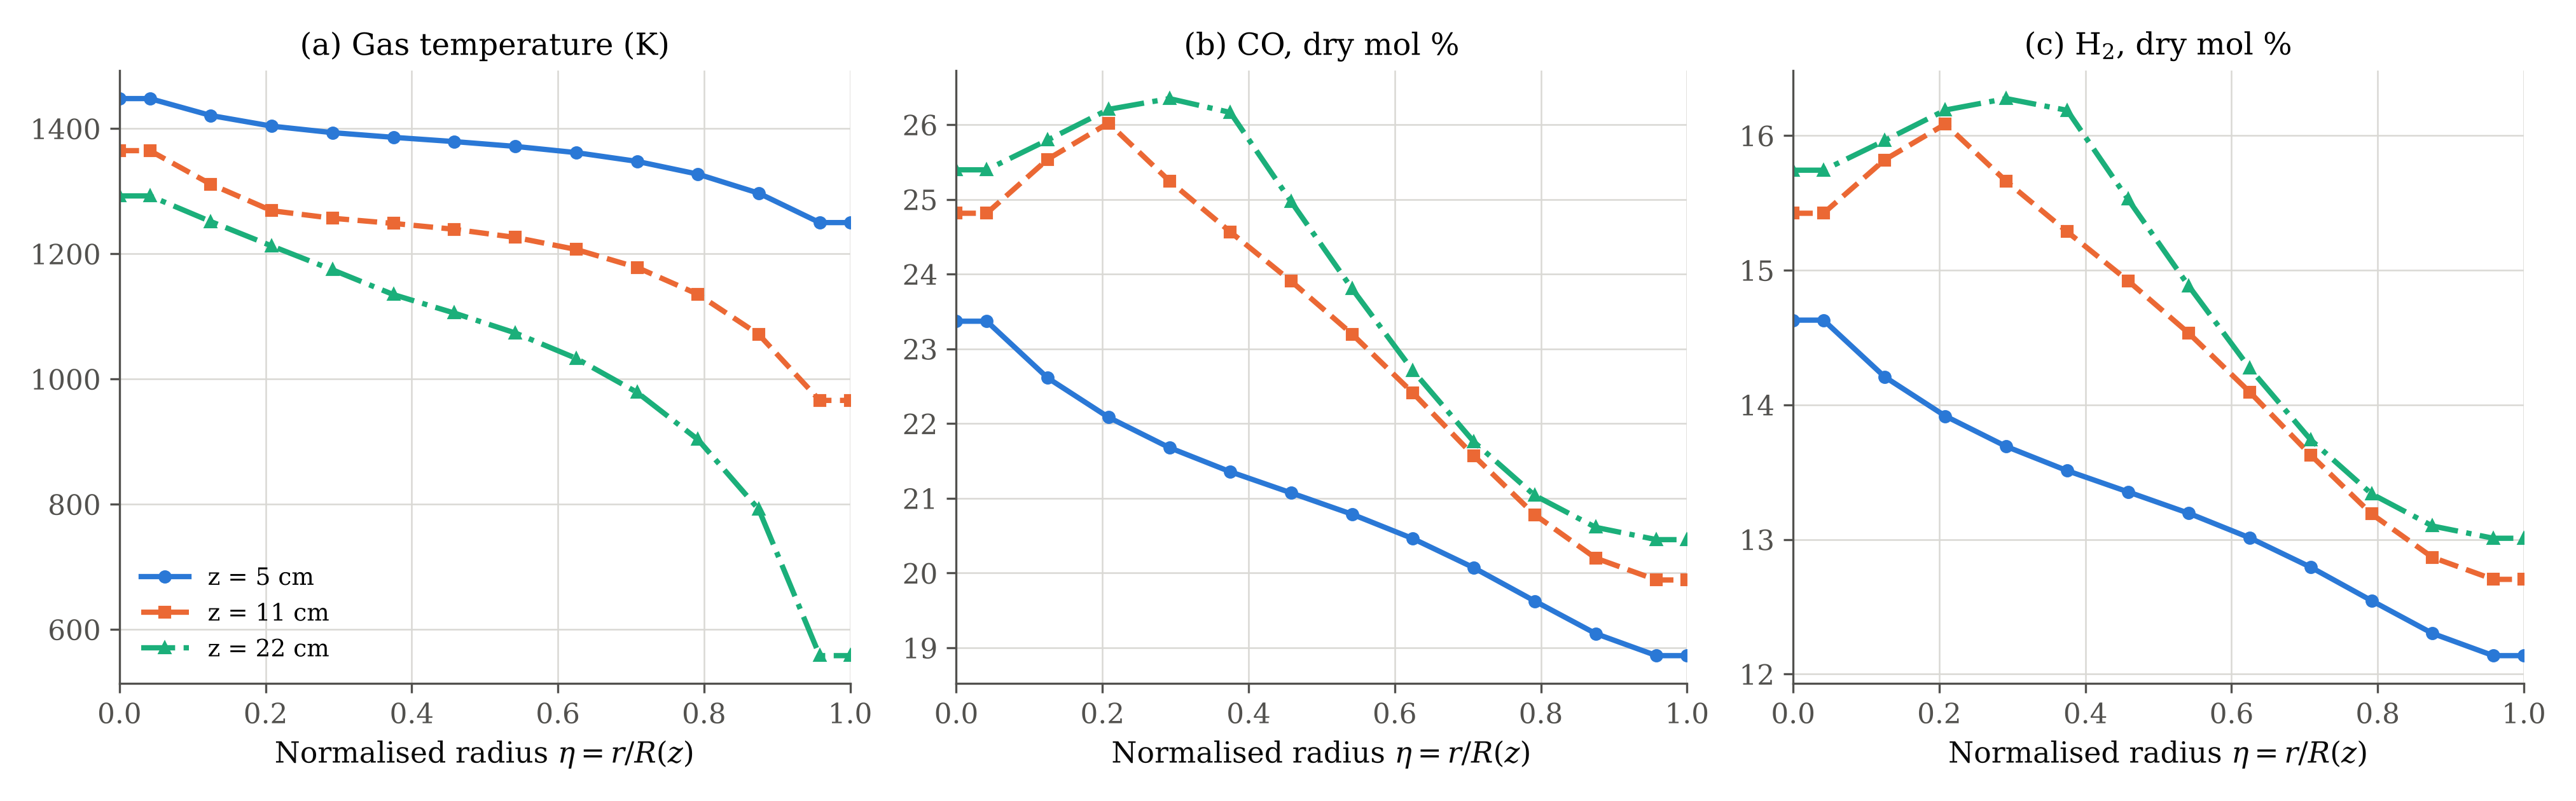
\includegraphics[width=\textwidth]{fig12_radial_profiles_2d.png}
\caption{Radial profiles from the 2D model at $z=5$, 11 and 22\,cm.}\label{fig:radial}
\end{figure}
Because heat leaves only through the wall, a cold boundary layer forms there. At 5\,cm the axis is at \RTwoDaxisTfive\,K and the wall cell at \RTwoDwallTfive\,K; at the exit the values are \RTwoDaxisTexit\,K and \RTwoDwallTexit\,K. Gasification consequently proceeds much further in the core than near the wall.

At the exit, CO is \RTwoDCOaxis\,\% on the axis but \RTwoDCOwall\,\% at the wall, and H$_2$ is \RTwoDHtwoaxis\ against \RTwoDHtwowall\,\%. Char on the axis is \RTwoDXcAxisFive\,\% converted by 5\,cm and \RTwoDXcAxisEleven\,\% by 11\,cm, but only \RTwoDXcWallExit\,\% near the wall. Once the core char is exhausted, the maximum CO and H$_2$ move slightly off the axis (Fig.~\ref{fig:radial}), where char is still reacting.

The flow-weighted exit gas of the 2D model (CO \RTwoDmixCO, H$_2$ \RTwoDmixHtwo, CO$_2$ \RTwoDmixCOtwo, N$_2$ \RTwoDmixNtwo\,\%) is richer than the 1D result. The 2D wall loss is lower (\RTwoDwallkW\ against \RWallkWRef\,kW) because the wall-side gas is colder. $U$ was calibrated with the 1D (mean-temperature) model, so the 2D results show the \emph{radial structure} of the hearth rather than a separately calibrated prediction.

%=====================================================================
\section{Validation against Jayah et al.\ (2003)}\label{sec:val}
\subsection{Calibration run (Jayah Table~5)}
\begin{table}[H]\centering\small
\caption{Jayah Table~5 run (2.5\,cm chips, Run~7 conditions). These data were \emph{used for calibration}, so the agreement is not independent evidence. Errors are in \%-points.}
\begin{tabular}{lrrrrr}
\toprule
Species (dry, \%) & Measured & Jayah model & This model & Error, this model & Error, Jayah\\
\midrule
\tabinput{generated/table_calibration.tex}
\midrule
MAE / RMSE & & & & \RCalMAE\ / \RCalRMSE & \RCalMAEJ\ / \RCalRMSEJ\\
\bottomrule
\multicolumn{6}{l}{\footnotesize \textsuperscript{a}CH$_4$ imposed at the throat in both models.}
\end{tabular}
\end{table}

\subsection{Nine experimental runs (Jayah Table~3): independent validation}
\begin{table}[H]\centering\small
\caption{Measured / simulated dry gas composition (\%) for the nine runs, with the simulated throat temperature. Feed rate assumed to be 18.6\,kg/h.}
\begin{tabular}{rrrrrcccc}
\toprule
Run & Chip (cm) & MC (\% d.b.) & AFR & $T_{g,0}$ (K) & CO & H$_2$ & CO$_2$ & N$_2$\\
\midrule
\tabinput{generated/table_ninerun_composition.tex}
\bottomrule
\end{tabular}
\end{table}
\begin{table}[H]\centering\small
\setlength{\tabcolsep}{4pt}\caption{Error statistics over the nine runs (\%-points; LHV in MJ/Nm$^3$). $R^2$ is about the 1:1 line; ``Std (meas.)'' is the run-to-run spread of the measurements.}
\begin{tabular}{lrrrrrrr}
\toprule
 & MAE & RMSE & Bias & Std (meas.) & $R^2$ & Within $\pm$10\,\% & MAE excl.\ Run 7\\
\midrule
\tabinput{generated/table_ninerun_stats.tex}
\bottomrule
\multicolumn{8}{l}{\footnotesize \textsuperscript{a}CH$_4$ is imposed, so its statistics do not test the model.}
\end{tabular}
\end{table}
\begin{figure}[H]\centering
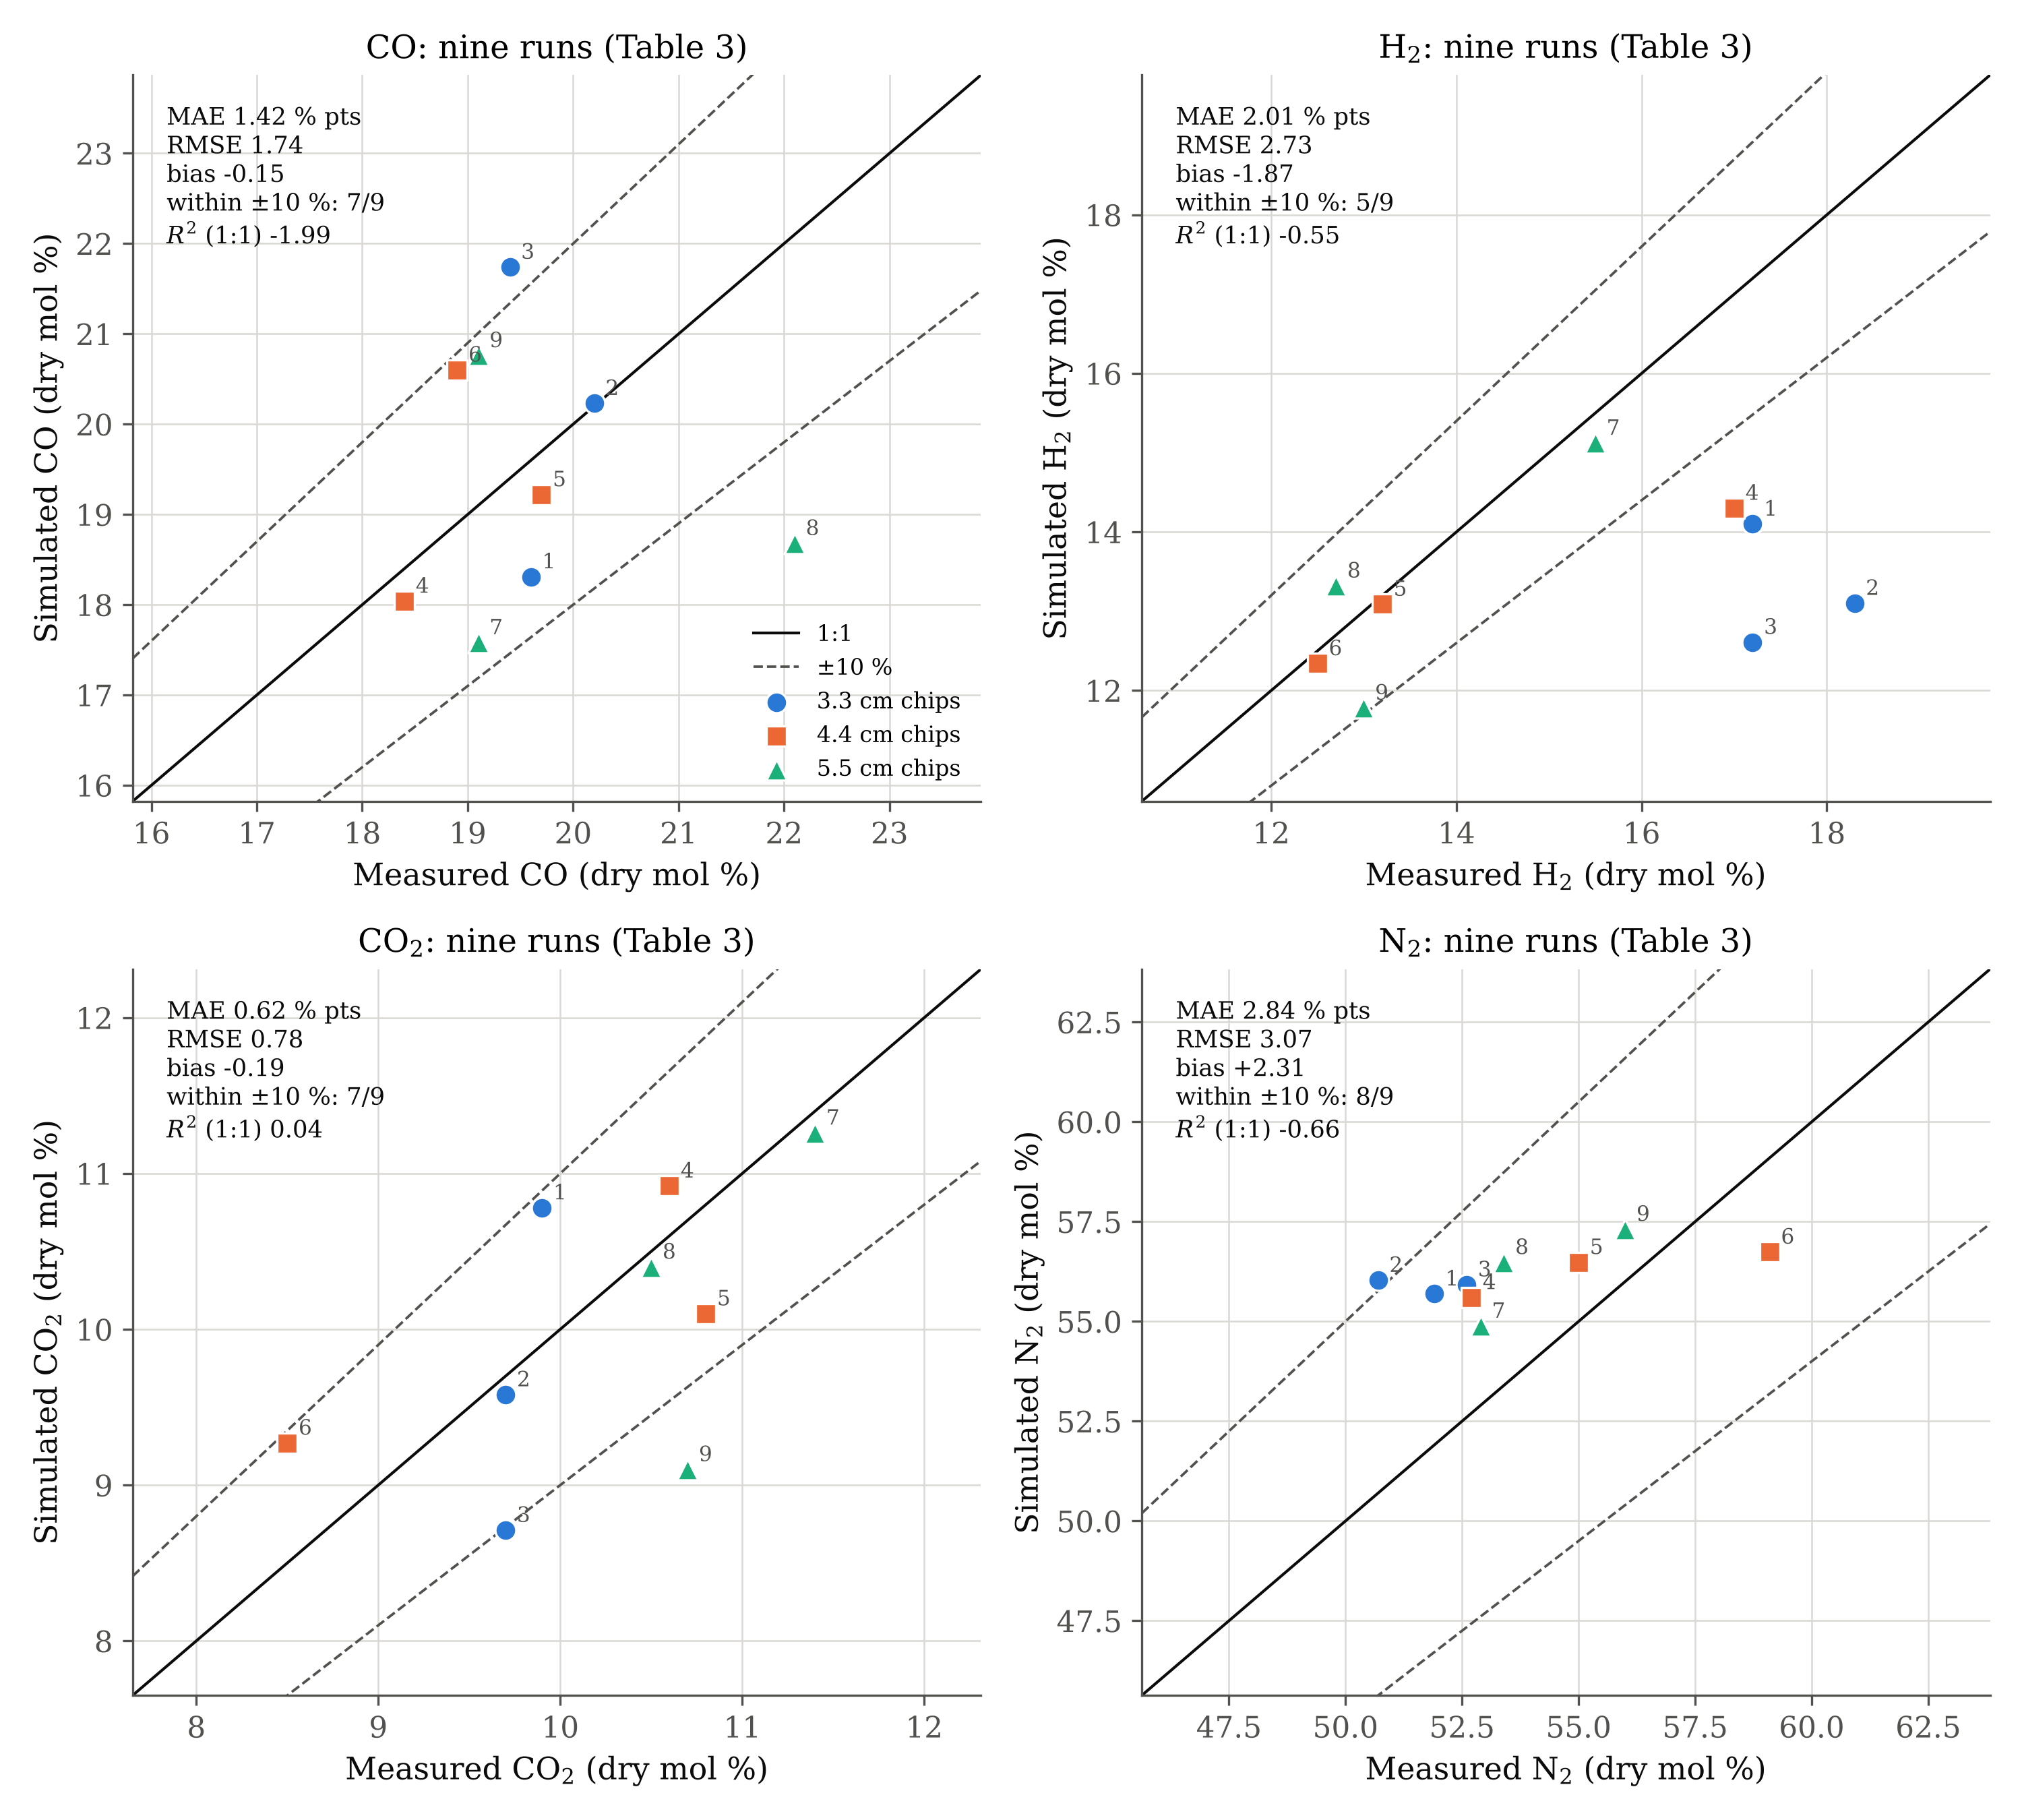
\includegraphics[width=0.82\textwidth]{fig09_validation_parity_plots.png}
\caption{Parity plots for the nine runs; points are labelled by run number. All statistics are computed in \texttt{src/validation.py}.}
\end{figure}

\paragraph{Interpretation.} The mean levels are reproduced well. CO has almost no bias (\RBiasCO\,\%-pts) and CO$_2$ is within \RMAECOtwo\,\%-pts on average, but two systematic problems remain:
\begin{itemize}
\item \textbf{H$_2$ is too low} (bias \RBiasHtwo\,\%-pts), mainly in Runs 1--4, where the measured H$_2$ is 17--18\,\%.
\item \textbf{N$_2$ is too high} (bias \RBiasNtwo), i.e.\ the model produces less gas per unit of air than the plant did.
\end{itemize}
The negative $R^2$ values do not mean the errors are large. The measured run-to-run spread is only 0.8--2.4\,\%-points, comparable with the model error, and the model does not capture which runs are richer. In the model, a higher AFR raises the throat temperature (Eq.~\ref{eq:anchor}) and with it CO. The data show no such trend: CO stays at 18.4--20.2\,\% for all AFRs, apart from Run 8 at 22.1\,\%.

Excluding Run~7, whose composition was the calibration target, changes the MAE only slightly (last column).

\subsection{Heating value and gas flow}
\begin{figure}[H]\centering
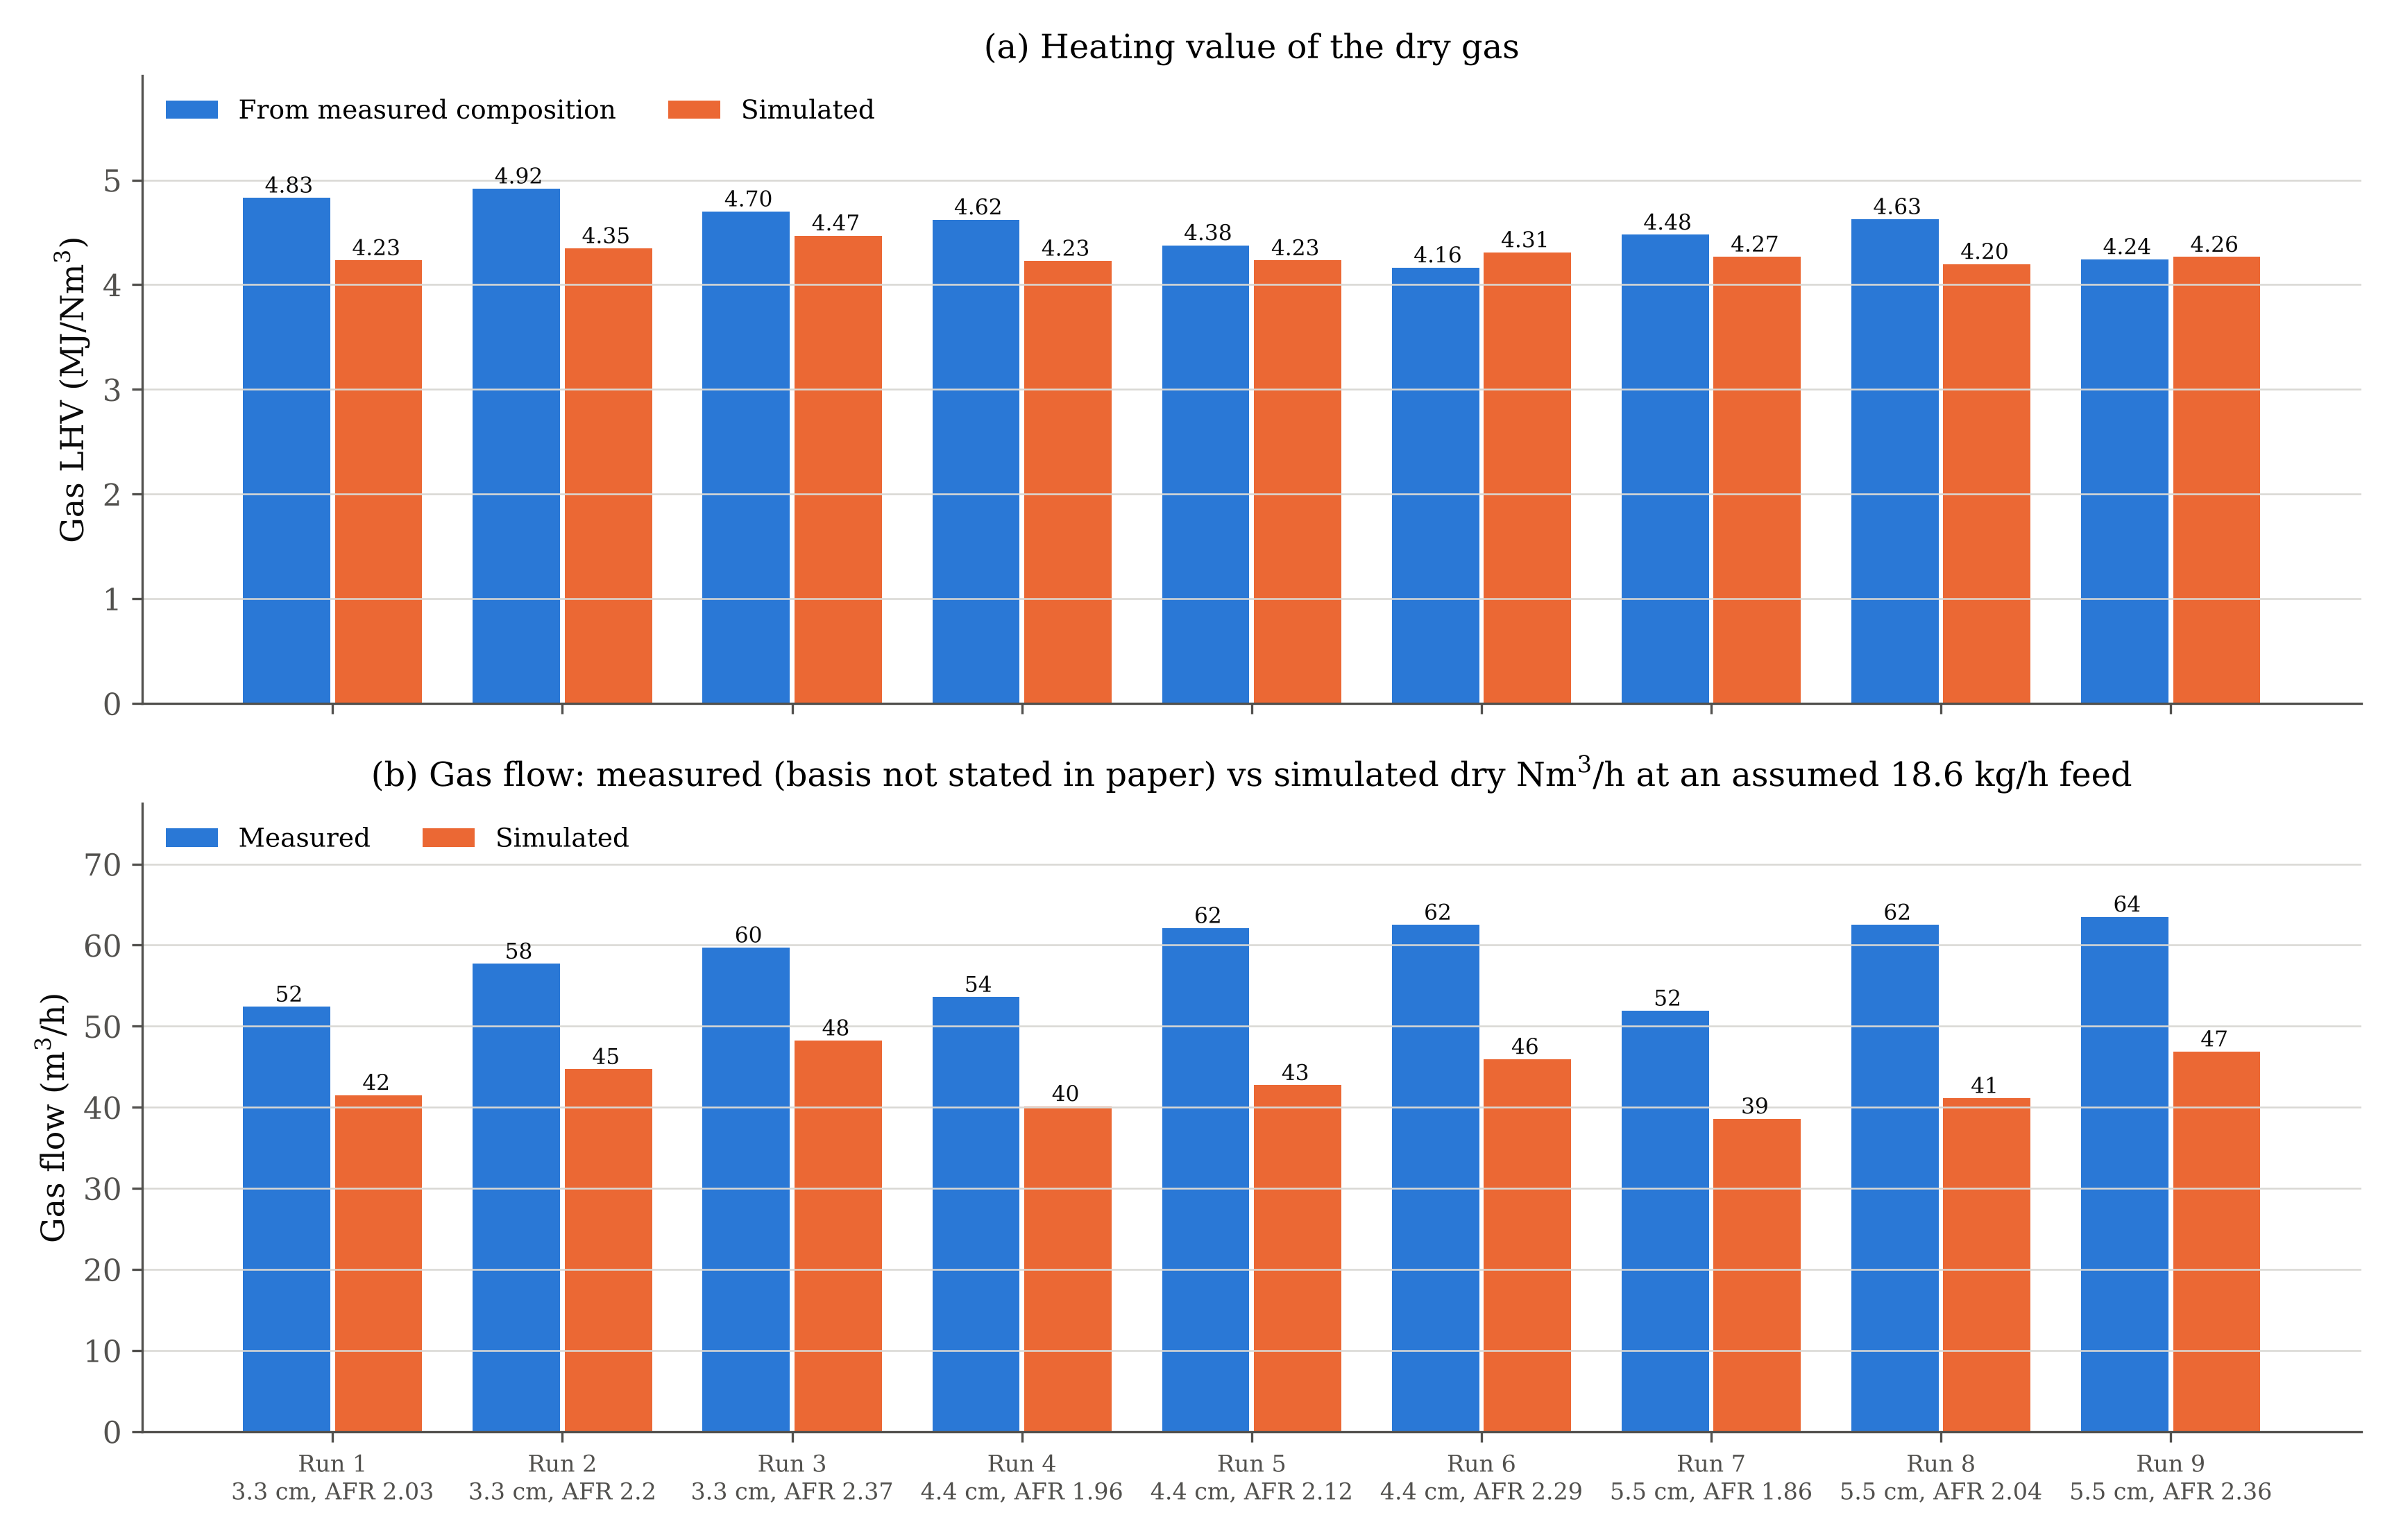
\includegraphics[width=0.9\textwidth]{fig10_principal_cases_comparison.png}
\caption{Gas LHV and gas flow per run.}
\end{figure}
\begin{table}[H]\centering\small
\caption{LHV, gas flow and conversion efficiency per run. ``Implied feed'' is the dry feed that would make the simulated flow equal to the measured one.}
\begin{tabular}{rrrrrrr}
\toprule
Run & \multicolumn{2}{c}{LHV (MJ/Nm$^3$)} & Flow meas. & Flow sim. & Implied feed & Efficiency\\
 & meas. & sim. & (m$^3$/h) & (Nm$^3$/h, dry) & (kg/h) & sim. (\%)\\
\midrule
\tabinput{generated/table_flow.tex}
\bottomrule
\end{tabular}
\end{table}
The LHV is predicted to within \RMAELHV\,MJ/Nm$^3$ on average (bias \RBiasLHV). The simulated dry flow is only \RFlowRatioMin--\RFlowRatioMax\,\% of the measured flow, but the comparison is weak. The paper does not state the basis of the measured flow (temperature, wet or dry), and it gives no feed rate for the individual runs. Because gas flow scales with feed, the shortfall corresponds to a dry feed of \RImpliedFeedMin--\RImpliedFeedMax\,kg/h instead of the assumed 18.6\,kg/h. Gas composition and LHV, being intensive, are almost unaffected by this assumption (Section~\ref{sec:sweeps}).

\subsection{Axial temperature (Jayah Fig.~5)}
\begin{table}[H]\centering\small
\caption{Gas temperature along the axis, AFR 2.20 (measured points and Jayah's model digitised from Jayah Fig.~5, $\pm$15\,K reading uncertainty).}
\begin{tabular}{rrrrrr}
\toprule
$z$ (cm) & Measured (K) & This model (K) & Error (K) & Jayah model (K) & Error (K)\\
\midrule
\tabinput{generated/table_temperature.tex}
\midrule
MAE / RMSE & & & \RTempMAE\ / \RTempRMSE & & \RTempMAEJ\ / \RTempRMSEJ\\
\bottomrule
\end{tabular}
\end{table}
Jayah Fig.~5 shows six measured points. Neither model was fitted to them. The present model is \RTempMAE\,K from the data on average (bias \RTempBias\,K), better than Jayah's model at \RTempMAEJ\,K. The largest errors are an over-prediction near the throat (4\,cm) and an under-prediction at 16--20\,cm, where the measured profile stays flat before dropping. Thermocouple readings in a reacting bed are themselves uncertain: they exchange radiation with the cooler wall and can be fouled by soot.

%=====================================================================
\section{Parametric study and engineering interpretation}
\subsection{Replication of Jayah et al.\ Table 7}
The base case is 3\,cm chips, 15\,\% d.b., AFR 2.20, air at 300\,K, a 61$^\circ$ throat and $U=\RUwall$\,W\,m$^{-2}$\,K$^{-1}$; one parameter is varied at a time. For the heat-loss cases, $U$ is re-solved so that the hearth loses 5, 10 or 15\,\% of the input. The optimum length follows Jayah's definition: the length at which efficiency reaches 99.5\,\% of its ultimate value.

\begin{figure}[H]\centering
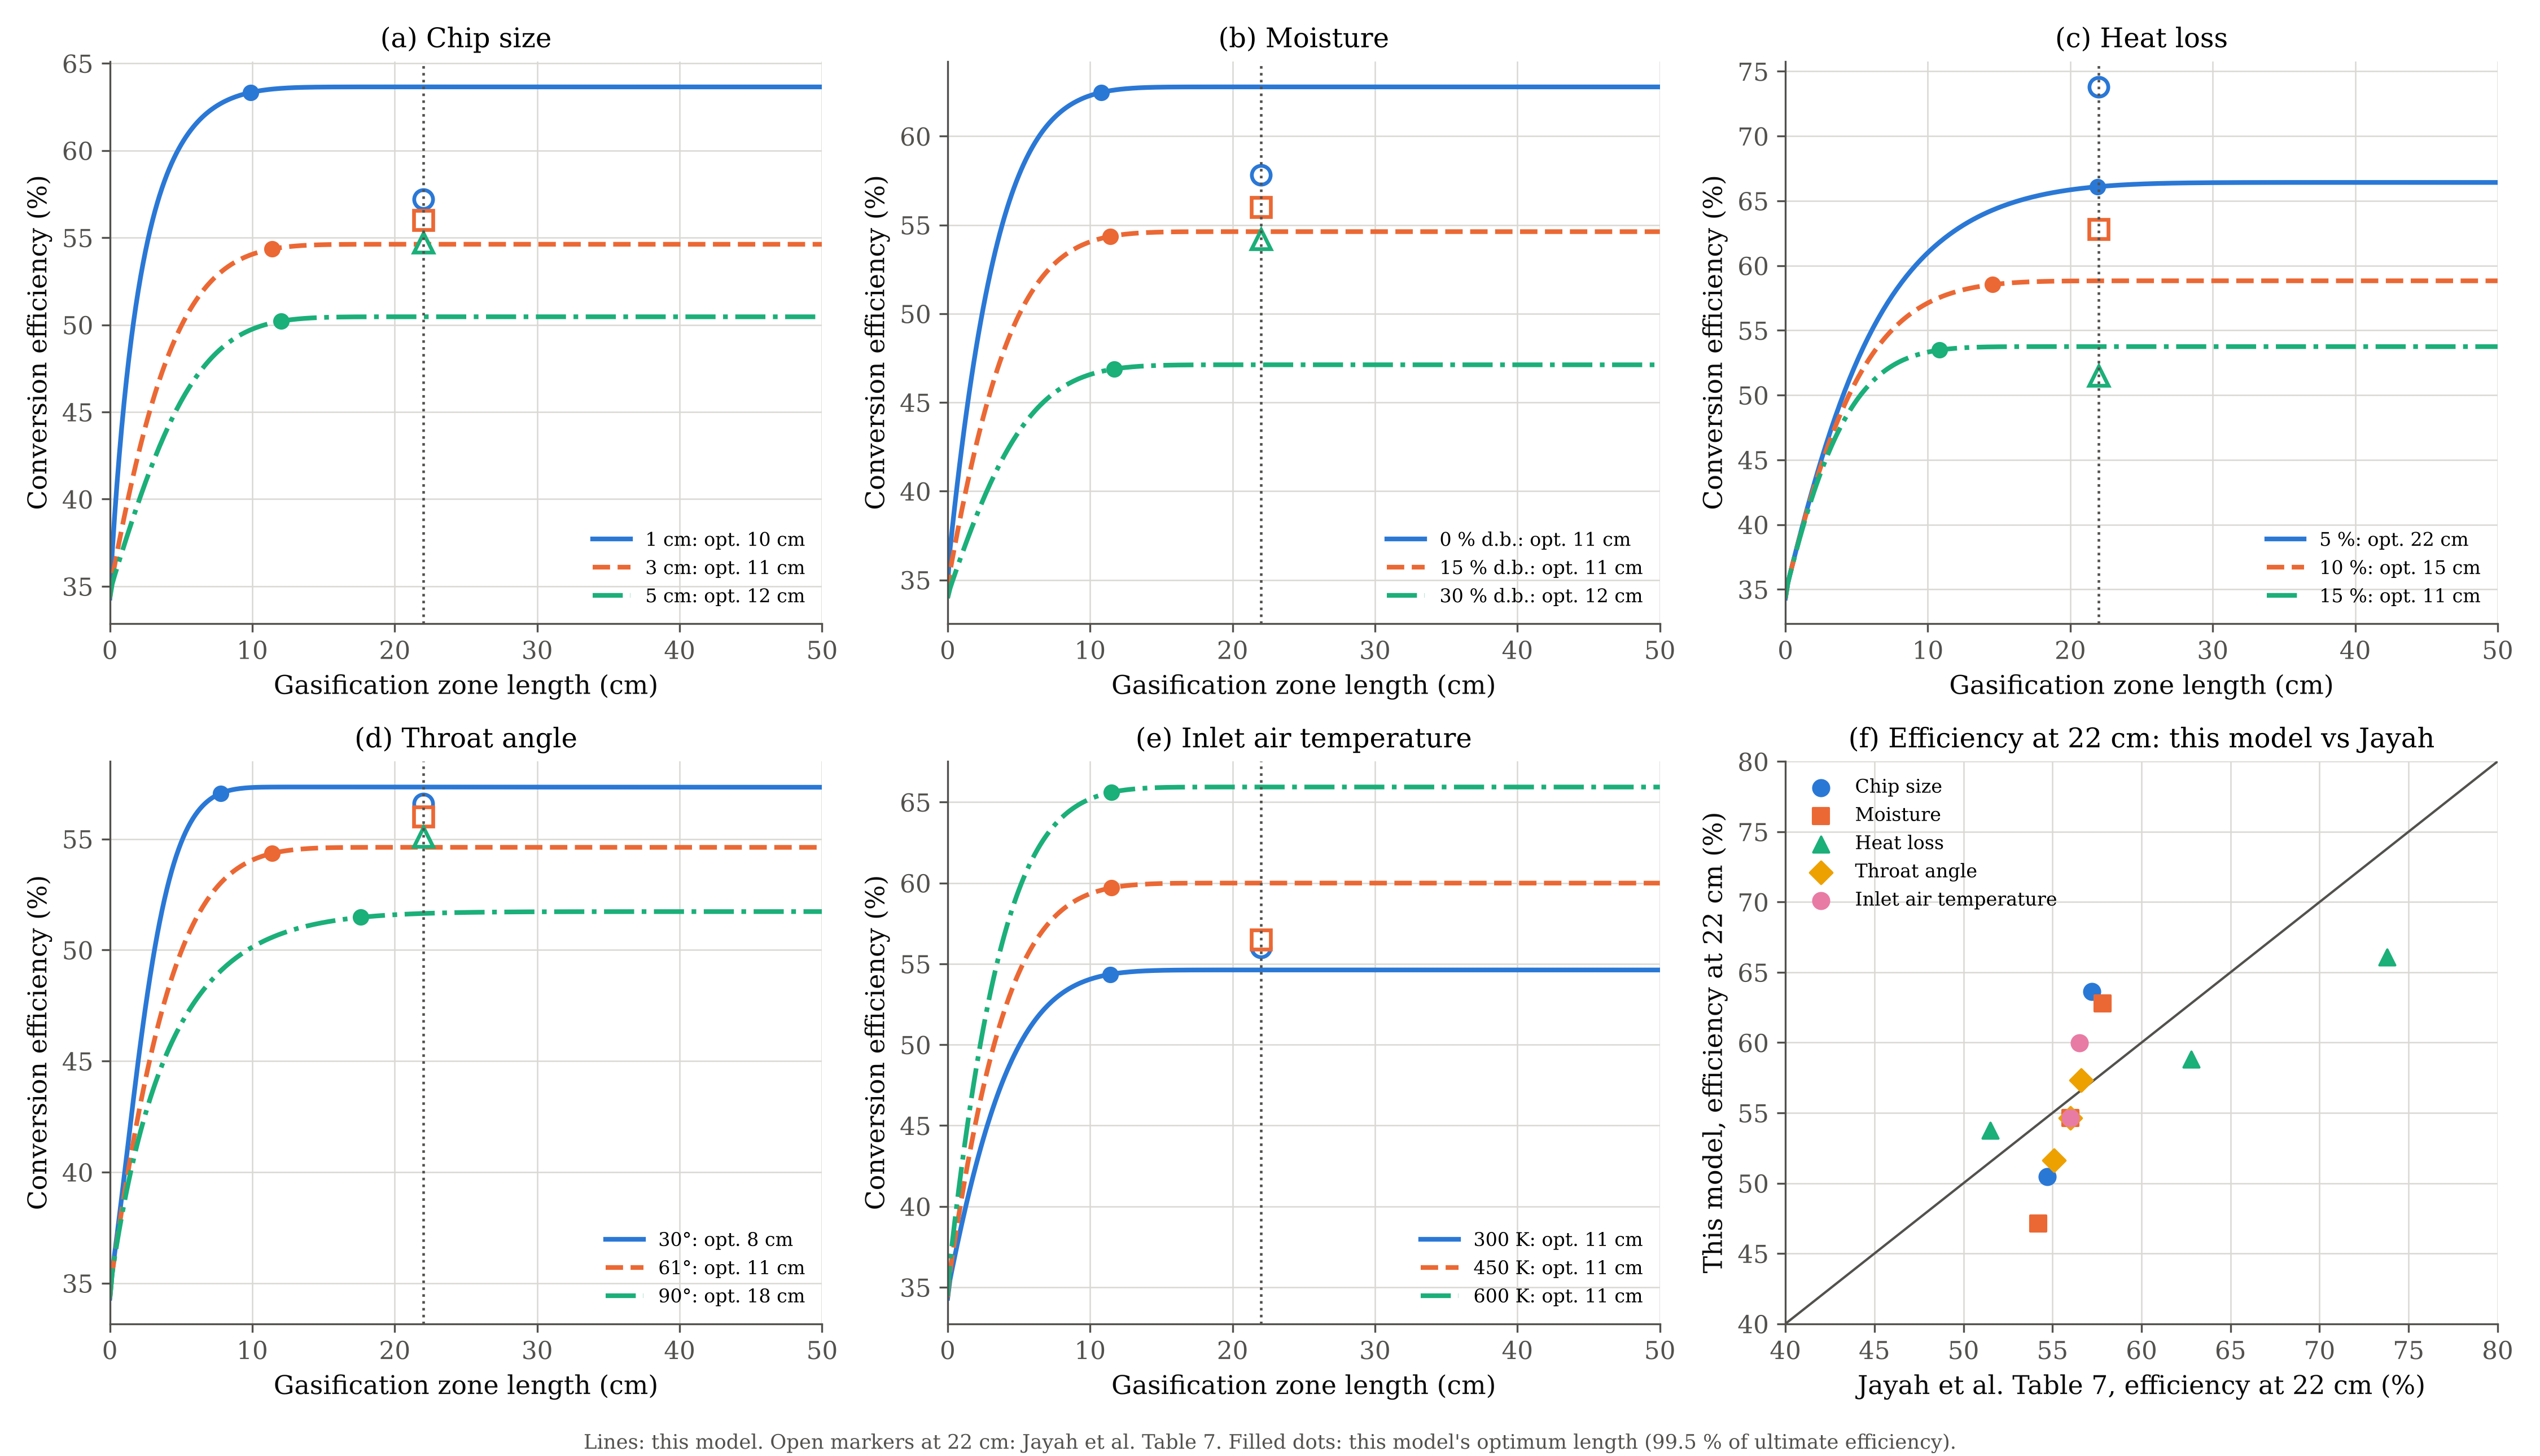
\includegraphics[width=\textwidth]{fig08_table7_replication.png}
\caption{Conversion efficiency vs.\ gasification-zone length (lines, this model) with Jayah's values at 22\,cm (open markers). Panel (f) compares the 22\,cm efficiencies directly.}
\end{figure}
\begin{table}[H]\centering\footnotesize\setlength{\tabcolsep}{4pt}
\caption{Comparison with Jayah et al.\ Table 7 (efficiency in \%, length in cm). The model's 61$^\circ$ case is compared with Jayah's 60$^\circ$ case; ``--'' means not reported.}
\begin{tabular}{llrrrrrrr}
\toprule
Parameter & Value & \multicolumn{2}{c}{Efficiency at 22 cm} & \multicolumn{2}{c}{Optimum length} & \multicolumn{2}{c}{Efficiency at optimum} & Hearth loss\\
 & & Model & Jayah & Model & Jayah & Model & Jayah & (\% input)\\
\midrule
\tabinput{generated/table_table7.tex}
\end{tabular}
\end{table}

\paragraph{What agrees.} The base-case efficiency at 22\,cm (\REffChipB\,\%) is close to Jayah's 56.0\,\%. Every trend has the right direction:
\begin{itemize}
\item smaller chips, drier wood, lower heat loss, a smaller throat angle and hotter air all raise efficiency;
\item heat loss is one of the two strongest levers (\REffLossA\,\% at 5\,\% loss against \REffLossC\,\% at 15\,\%; Jayah: 73.8 to 51.5\,\%).
\end{itemize}

\paragraph{What differs.}
\begin{itemize}
\item \textbf{Moisture, chip size and air temperature act more strongly in this model.} 0--30\,\% moisture gives \REffMCA--\REffMCC\,\% (Jayah 57.8--54.2\,\%). Pre-heating air to 450\,K adds 5\,\%-points (Jayah: 0.5). These effects act through the throat temperature (Eq.~\ref{eq:anchor}) and the strongly temperature-dependent char kinetics, and the size of the response depends on the assumed anchoring.
\item \textbf{The optimum length is much shorter: \ROptChipB\,cm instead of 32--33\,cm.} With 12.8\,\% of the input lost through an uninsulated hearth, the bed has cooled to \RBaseTtwelve\,K by 12\,cm, where the char reactions (activation energies of about 240\,kJ/mol) have effectively stopped. Lengthening the hearth then only adds wall area. Only when the loss is cut to 5\,\% does the optimum move out to the present 22\,cm (\ROptLossA\,cm), with efficiency rising to \REffLossA\,\%.
\end{itemize}

\paragraph{Design implication.} This model does not support lengthening the hearth to 33\,cm on its own. It agrees with Jayah et al.\ that reducing heat loss (insulating the reactor) is the most effective change. With better insulation, the existing 22\,cm hearth is close to the optimum length.

\subsection{Air--fuel ratio and feed rate}\label{sec:sweeps}
\begin{figure}[H]\centering
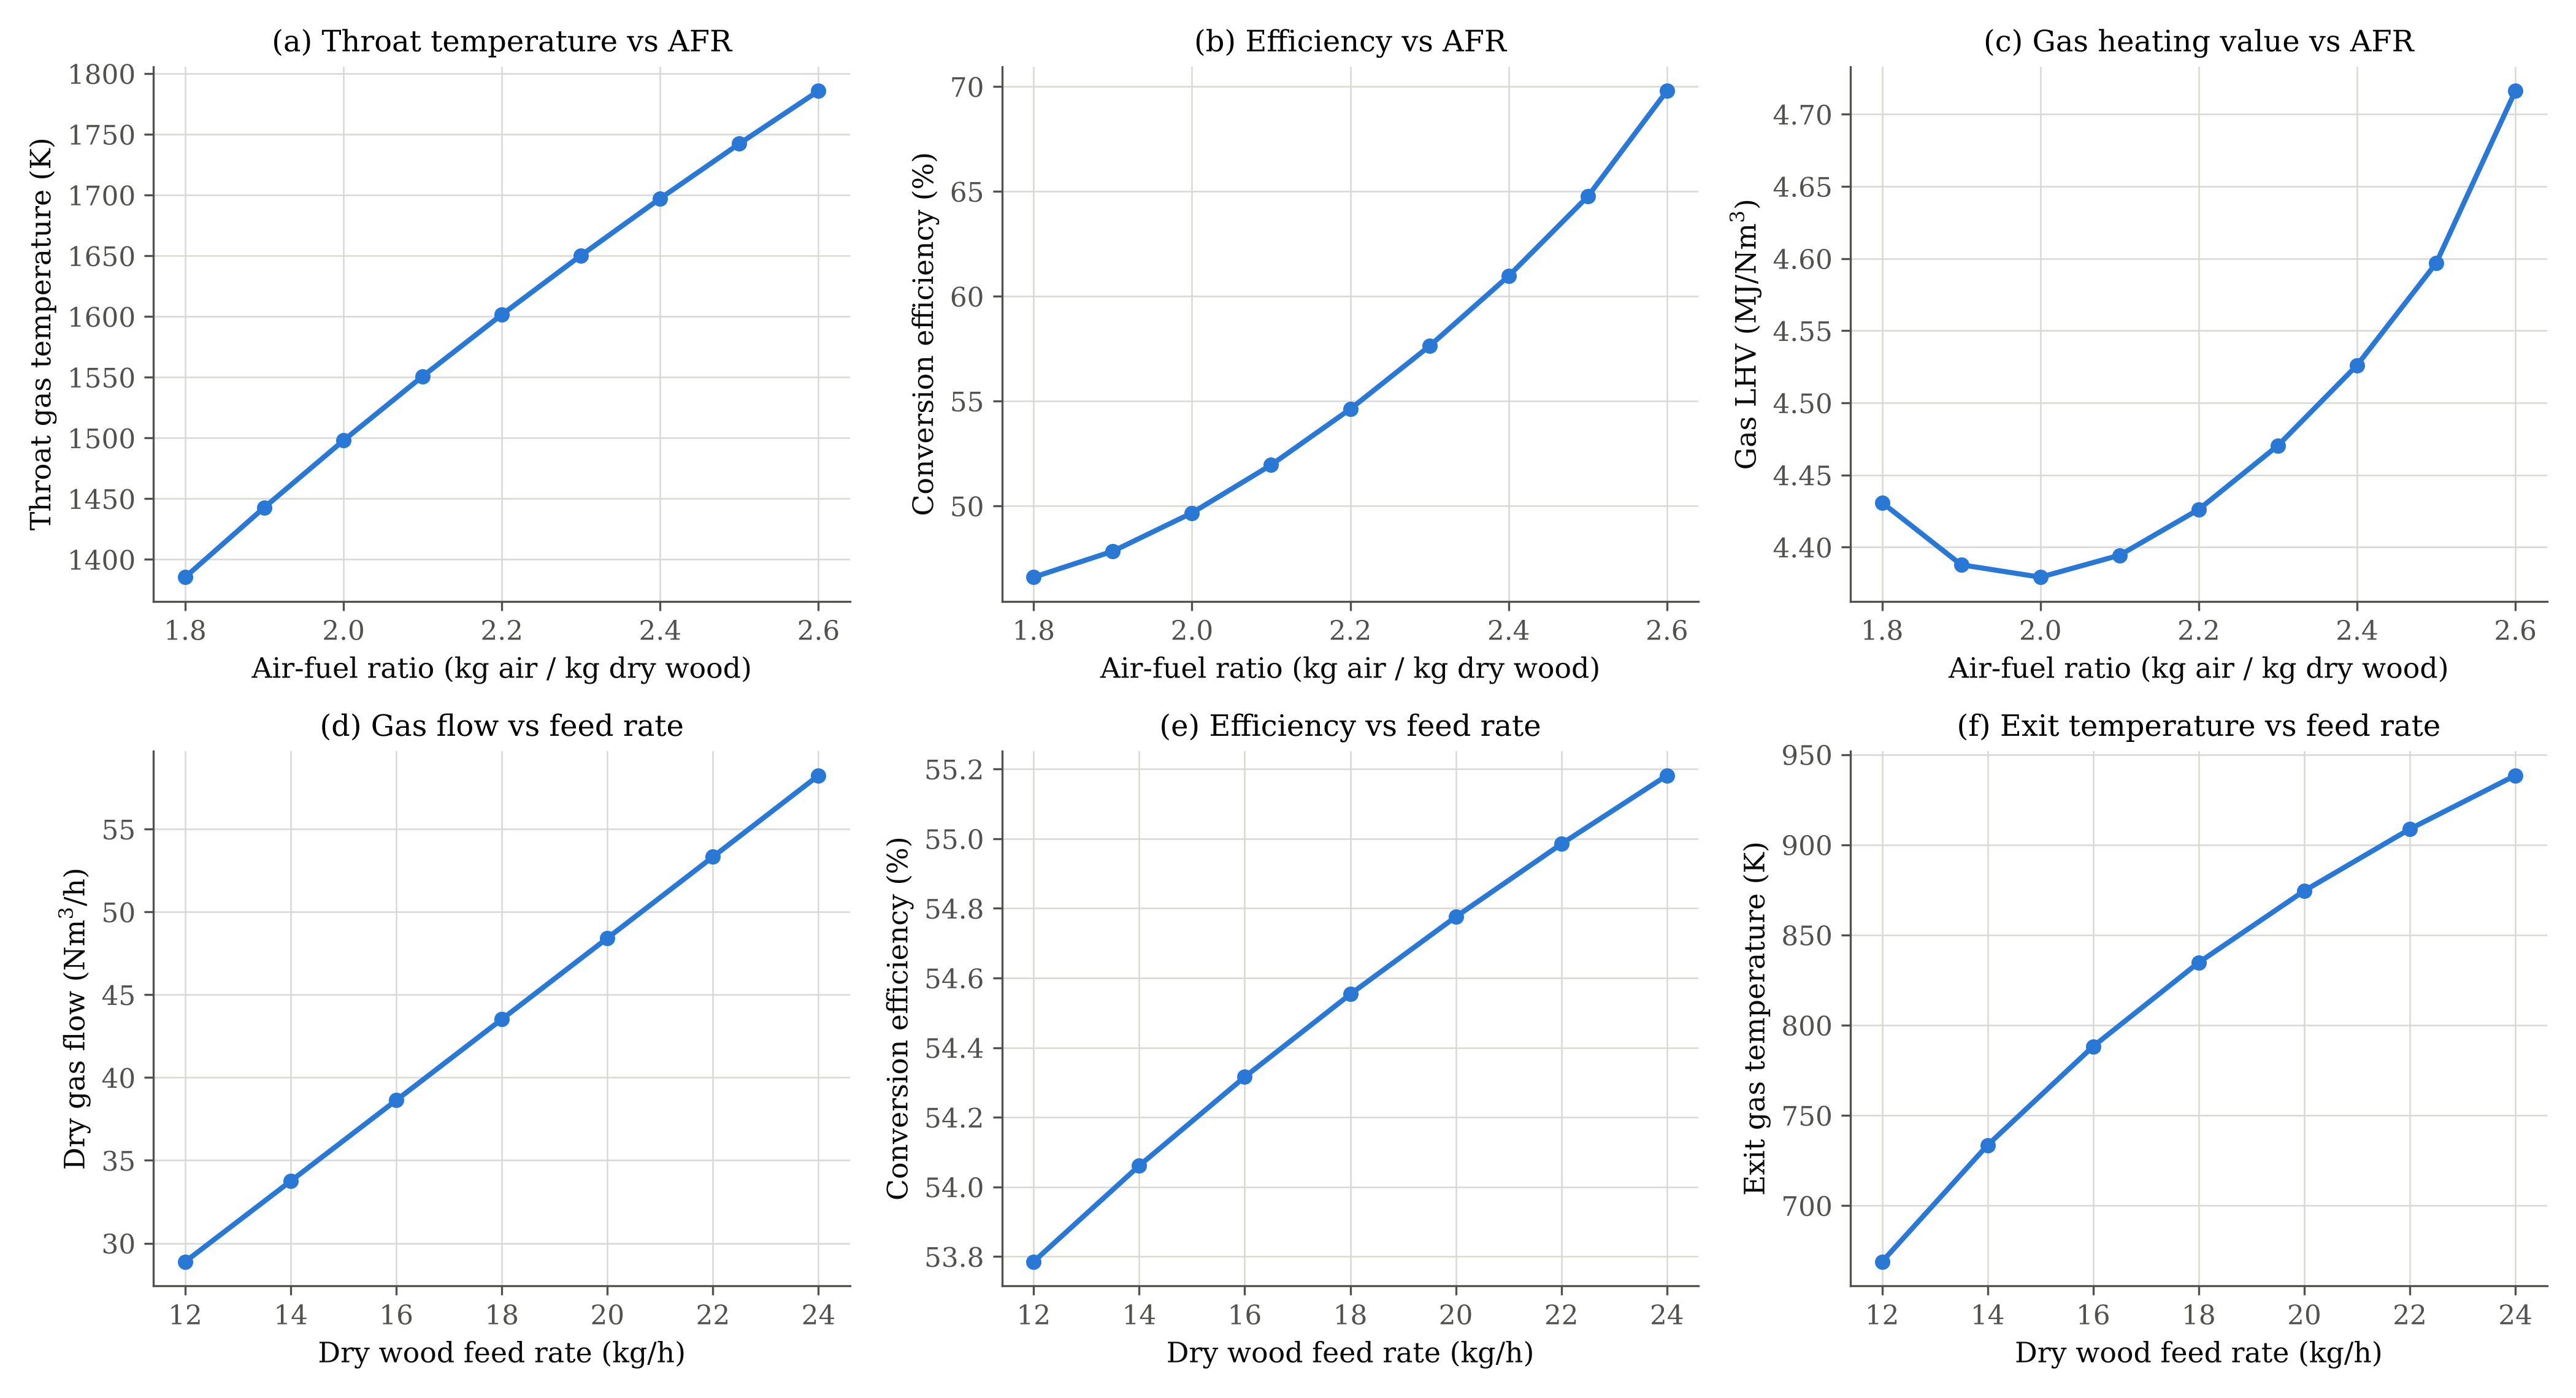
\includegraphics[width=\textwidth]{fig11_operating_sweeps.png}
\caption{Effect of air--fuel ratio and dry feed rate at 22\,cm (3\,cm chips, 15\,\% d.b.).}
\end{figure}
\begin{itemize}
\item \textbf{Air--fuel ratio.} Raising AFR from 1.8 to 2.6 raises the throat temperature from \RAFRTlo\ to \RAFRThi\,K. Char conversion rises from \RAFRXclo\ to \RAFRXchi\,\% and efficiency from \RAFRCGElo\ to \RAFRCGEhi\,\%, while the gas LHV stays within \RAFRLHVmin--\RAFRLHVmax\,MJ/Nm$^3$. In this model efficiency keeps rising until the char is used up near AFR 2.6 (ER 0.42). Real gasifiers usually peak earlier because extra air burns product gas, which the throat sub-model represents only through equilibrium. This trend should be treated with caution beyond the tested range of AFR 1.86--2.37.
\item \textbf{Feed rate.} Gas flow scales almost linearly with feed (\RFeedFlowLo\ to \RFeedFlowHi\,Nm$^3$/h for 12--24\,kg/h). Efficiency changes little (\RFeedCGElo--\RFeedCGEhi\,\%), and the exit temperature rises from \RFeedTlo\ to \RFeedThi\,K because a fixed wall loss becomes a smaller fraction of a larger throughput.
\end{itemize}

%=====================================================================
\section{Limitations and uncertainty}\label{sec:lim}
\begin{enumerate}
\item \textbf{Throat temperature anchoring.} A mixed enthalpy balance gives about 1345\,K at the reference condition. The model instead uses Jayah's $\approx$1604\,K plus the balance-predicted \emph{change}. The absolute throat temperature, and the size of the AFR, moisture and air-temperature effects, carry this assumption.
\item \textbf{Water-gas-shift rate.} The units of the literature expression are ambiguous. The fast interpretation would give a very different gas (Section~\ref{sec:kin}).
\item \textbf{Calibration.} Three parameters are fitted: $U$ to the 12.8\,\% loss, and $\eta_\text{B}$, $\eta_\text{WG}$ to Jayah Table~5. The large effective $U$ concentrates all measured loss in the hearth. The calibration run converts only \RCalXc\,\% of its char, below the 41--80\,\% implied by Jayah Table~4.
\item \textbf{Data gaps and inconsistencies in the paper.} Per-run feed rates and the basis of the measured gas flow are not given. Jayah Table~5 (2.5\,cm) and Jayah Table~3 (Run~7, 5.5\,cm) disagree on chip size. The chip size and moisture of the Jayah Fig.~5 trial are not stated. Jayah Table~4 implies an air--fuel ratio of about 3.0, outside Jayah Table~3's range.
\item \textbf{CH$_4$ and tar.} Methane is imposed rather than predicted. Tar is not modelled; it falls within Jayah's 7--9\,\% ``unaccounted'' material.
\item \textbf{2D model.} It resolves radial heat and species dispersion only. Velocity profiles, wall channelling, nozzle jets and bed bridging are not represented, and it is not CFD.
\item \textbf{Run-to-run variation.} The model does not reproduce the measured variation between runs ($R^2\le0$).
\end{enumerate}

%=====================================================================
\section{Conclusions}
\begin{enumerate}
\item The model was built from the paper's feedstock data (Jayah Tables~1--2), geometry and run conditions. It reproduces the calibration gas to \RCalMAE\,\%-points (Jayah's model: \RCalMAEJ).
\item Against the nine independent runs, the mean errors are \RMAECO\ (CO), \RMAEHtwo\ (H$_2$) and \RMAECOtwo\ (CO$_2$) \%-points, and \RMAELHV\,MJ/Nm$^3$ in LHV. H$_2$ is biased low and the run-to-run differences are not captured.
\item The axial gas temperature matches the six Jayah Fig.~5 measurements to \RTempMAE\,K, better than Jayah's own model (\RTempMAEJ\,K). The gas and char equilibrate within about \RzEquil\,cm of the throat.
\item The 2D model shows a hot core and a cold wall layer (\RTwoDaxisTexit\ against \RTwoDwallTexit\,K at the exit). Core char is exhausted by about 11\,cm while near-wall char is barely converted, so CO and H$_2$ are richest in the core.
\item The parametric study agrees with Jayah et al.\ on the direction of every effect and on heat loss being decisive. It disagrees on the optimum length: with 12.8\,\% loss, conversion stops after about 11--12\,cm, so insulating the hearth, not lengthening it, is the recommended improvement.
\end{enumerate}
\textbf{Future work:} measure per-run feed rate and gas flow on a stated basis; resolve the WGS kinetics and throat temperature with a non-premixed flame sub-model; add tar kinetics and a velocity/channelling model to the 2D formulation.

%=====================================================================
\section*{References}
\begin{enumerate}[label={[\arabic*]},leftmargin=*]
\item Jayah T.H., Aye L., Fuller R.J., Stewart D.F. (2003). Computer simulation of a downdraft wood gasifier for tea drying. \emph{Biomass and Bioenergy} 25(5), 459--469.
\item Chen J.S. (1987). \emph{Kinetic engineering modelling of co-current moving bed gasification reactors for carbonaceous material}. PhD thesis, Cornell University.
\item Milligan J.B. (1994). \emph{Downdraft gasification of biomass}. PhD thesis, Aston University.
\item Groeneveld M.J., van Swaaij W.P.M. (1980). Gasification of char particles with CO$_2$ and H$_2$O. \emph{Chemical Engineering Science} 35, 307--313.
\item Yoon H., Wei J., Denn M.M. (1978). A model for moving-bed coal gasification reactors. \emph{AIChE Journal} 24(5), 885--903.
\item Ranz W.E., Marshall W.R. (1952). Evaporation from drops. \emph{Chemical Engineering Progress} 48, 141--146 and 173--180.
\item Wakao N., Funazkri T. (1978). Effect of fluid dispersion coefficients on particle-to-fluid mass transfer coefficients in packed beds. \emph{Chemical Engineering Science} 33, 1375--1384.
\item Zainal Z.A., Rifau A., Quadir G.A., Seetharamu K.N. (2002). Experimental investigation of a downdraft biomass gasifier. \emph{Biomass and Bioenergy} 23(4), 283--289.
\end{enumerate}

%=====================================================================
\appendix
\section{Model parameters}
\begin{table}[H]\centering\footnotesize
\caption{Parameters as used in \texttt{src/config.py}.}\label{tab:params}
\begin{tabular}{llll}
\toprule
Symbol & Description & Value & Status\\
\midrule
$U$ & wall heat-loss coefficient & \RUwall\ W\,m$^{-2}$\,K$^{-1}$ & calibrated (12.8\,\% loss)\\
$\eta_\text{B}$ & Boudouard effectiveness factor & \RetaB & calibrated (Jayah Table~5)\\
$\eta_\text{WG}$ & water-gas effectiveness factor & \RetaWG & calibrated (Jayah Table~5)\\
$A_1$, $E_1$ & Boudouard intrinsic constants & $3.616\times10^{8}$, 240 kJ/mol & as implemented\\
$A_2$, $E_2$ & water-gas intrinsic constants & $1.517\times10^{9}$, 241 kJ/mol & as implemented\\
$A_3\eta_3$, $E_3$ & methanation & $4.189\times10^{3}\times0.05$, 130 kJ/mol & as implemented\\
$k_4$ & water-gas shift & $2.78\times10^{-3}\,e^{-1510/T}$ m$^3$/(mol\,s) & assumption (units)\\
$T_\text{anchor}$ & throat temperature at AFR 2.20 & 1604 K & Jayah Fig.~5 (digitised)\\
$\varepsilon$ & bed voidage & 0.48 & assumption\\
$\rho_\text{char}$ & char particle density & 250 kg/m$^3$ & assumption\\
CH$_4$ at throat & dry mole fraction & 1.2\,\% & imposed (as in Jayah)\\
$Pe_m$, $Pe_h$ & radial P\'eclet numbers (2D) & 10, 8 & packed-bed values\\
\bottomrule
\end{tabular}
\end{table}
Because the rates are calibrated through $\eta_j$, the individual intrinsic pre-exponential factors are not claimed as independent literature values; only the products $\eta_j A_j$ are constrained by the data.

\section{Reproducing the results}
\begin{verbatim}
pip install -r requirements.txt
python run_simulation.py              # all figures and tables (~30 s)
python -m pytest tests                # 20 tests
python -m src.calibration             # re-derive U, eta_B, eta_WG
python scripts/make_report_tables.py  # regenerate report numbers
\end{verbatim}
Every simulated number in this report is generated from the files in \texttt{outputs/tables} by the script \texttt{make\_report\_tables.py} in \texttt{scripts}; none are typed by hand.

\end{document}
